\documentclass[12pt,reqno]{amsart}
\usepackage[margin=3cm]{geometry}

\usepackage{amsmath, amssymb, amsfonts, tikz,enumerate, graphicx, textcomp, caption, wrapfig, amsthm, todonotes, verbatim, cleveref, caption, float, mathabx, flafter}
\usetikzlibrary{calc, arrows}
\usepackage[procnames]{listings}
\usepackage{color, subfig}
\usepackage[section]{placeins}

\usepackage{color}
\definecolor{purple}{rgb}{0.5,0,1}

\newenvironment{dami}{
  \medskip
\begin{color}{blue}
    \textcolor{purple}{\textbf{Dami:}} 
}{
\end{color}
  \medskip
}


\newenvironment{cat}{
  \medskip
\begin{color}{red}
    \textcolor{red}{\textbf{Catherine:}} 
}{
\end{color}
  \medskip
}

\definecolor{keywords}{RGB}{255,0,90}
\definecolor{comments}{RGB}{0,0,113}
\definecolor{red}{RGB}{160,0,0}
\definecolor{green}{RGB}{0,150,0}
\lstdefinelanguage{Magma}%
  {%
   otherkeywords={:=,+:=,-:=,*:=},%
          % functions
   procnamekeys={function,func,intrinsic,procedure,proc},%
         % Booleans
   morekeywords={true,false},%
          % relations
   morekeywords=[2]{adj,and,cat,cmpeq,cmpne,diff,div,eq,ge,gt,in,is,join,le,lt,%
          meet,mod,ne,notadj,notin,notsubset,or,sdiff,subset,xor},%
          % keywords
   morekeywords=[3]{assigned,break,by,case,catch,continue,declare,default,%
          delete,do,elif,else,end,eval,exists,exit,for,forall,fprintf,if,local,%
          not,print,printf,quit,random,read,readi,repeat,restore,save,select,%
          then,time,to,try,until,vprint,vprintf,vtime,when,where,while},%
          % directives
   morekeywords=[4]{clear,forward,freeze,iload,import,load},%
          % error checks
   morekeywords=[5]{assert,assert2,assert3,error,require,requirege,requirerange},%
          % constructors
   morekeywords=[6]{car,comp,cop,elt,ext,frac,hom,ideal,iso,lideal,loc,map,%
          ncl,pmap,quo,rec,recformat,rep,rideal,sub},%
          % other constructors (semi-reserved)
   morekeywords=[7]{AbelianGroup,AdditiveCode,AffineAlgebra,Algebra,%
          AssociativeAlgebra,Character,CliffordAlgebra,Design,Digraph,%
          ExtensionField,FPAlgebra,FiniteAffinePlane,FiniteProjectivePlane,%
          Graph,Group,GroupAlgebra,IncidenceStructure,LieAlgebra,LinearCode,%
          LinearSpace,MatrixAlgebra,MatrixGroup,MatrixRing,Monoid,%
          MultiDigraph,MultiGraph,NearLinearSpace,Network,PartialMap,%
          PermutationGroup,PolycyclicGroup,QuaternionAlgebra,Semigroup,%
          ZModule},%
          % functions
   morekeywords={[8]function,func,intrinsic,procedure,proc,return},%
      sensitive,%
      morecomment=[l]//,%
      morecomment=[s]{/*}{*/},%
      morecomment=[s]{\{}{\}},%
      morestring=[b]"%
  }[keywords,procnames,comments,strings]%
\lstset{language=Python, 
        basicstyle=\ttfamily\small, 
        keywordstyle=\color{keywords},
        commentstyle=\color{comments},
        stringstyle=\color{red},
        breaklines=true,
        showstringspaces=false,
        identifierstyle=\color{green},
        procnamekeys={def,class}}
%\usepackage[T1]{fontenc}
%\usepackage[urw-garamond]{mathdesign}
\usepackage{tikz-cd}\tikzset{node distance=2cm, auto}
\DeclareMathOperator{\Aut}{Aut}
\DeclareMathOperator{\Hom}{Hom}
\DeclareMathOperator{\Jac}{Jac}
\DeclareMathOperator{\Alt}{Alt}
\DeclareMathOperator{\Corr}{Corr}
\DeclareMathOperator{\im}{im}
\DeclareMathOperator{\uncurry}{uncurry}
\DeclareMathOperator{\Pic}{Pic}
\DeclareMathOperator{\Div}{Div}
\newcommand{\C}{\mathbb{C}}
\newcommand{\Z}{\mathbb{Z}}
\newcommand{\F}{\mathbb{F}}
\newcommand{\G}{\mathbb{G}}
\newcommand{\Q}{\mathbb{Q}}
\newcommand{\R}{\mathbb{R}}
\newcommand{\n}{\newline}
\newcommand{\mc}{\mathcal}
\newcommand{\te}{\text}
\newcommand{\bb}{\mathbb}
\renewcommand{\P}{\mathbb{P}}
\newcommand{\BBF}{\overline{\F_p}}
\newcommand\mapsfrom{\mathrel{\reflectbox{\ensuremath{\mapsto}}}}
\definecolor{codegray}{gray}{0.9}
\newcommand{\code}[1]{\colorbox{codegray}{\texttt{#1}}}
\newtheorem{theorem}{Theorem}
\newtheorem*{thm*}{Theorem}
\newtheorem*{proposition}{Proposition}
\newtheorem{lemma}[theorem]{Lemma}
\newtheorem*{lemma*}{Lemma}
\newtheorem*{qlemma*}{``Lemma"}
\newtheorem{cor}[theorem]{Corollary}
\newtheorem{conjecture}[theorem]{Conjecture}
\newtheorem{postulate}[theorem]{Postulate}
\newtheorem*{question}{Question}
\theoremstyle{definition}
\newtheorem{defn}{Definition}
\newtheorem{example}[theorem]{Example}
\theoremstyle{remark}
\newtheorem*{remark}{Remark}
\newtheorem*{notation}{Notation}
\newtheorem*{note}{Note}
\newcommand{\sss}{\ss$\text{ }$}
\newcommand{\ti}{\todo[inline]}
\newcommand{\DD}{\Delta\kern -8.3pt {\diamond} \kern -4.5pt \cdot \:}
\newenvironment{myproof}[1][``\proofname '']{%
  \proof[ #1]%
}{\endproof}


\title{The Study of Principal Polarizations through Automorphisms of Abelian Varieties} 
\author{Dami Lee and Catherine Ray}

\begin{document}

	
\maketitle

\begin{abstract} 
\end{abstract}

%todo: 
%rearrange
%correct grammatical errors
%read lange's latest paper and add to intro
%why is Narasimhan Nori important? -- unsolved as fuck. 

\section{Introduction}

Our paper introduces a new computer program to find multiple non-isomorphic principal polarizations on abelian varieties in characteristic 0, the code for which is publically available. In general, abelian varieties with several principal polarizations are incredibly rare. In fact, abelian varieties with no principal polarizations are, in some sense, dense on the moduli stack of abelian varieties. %(considered in terms of their big Period matrix).

The fact that an abelian variety admits only a finite number of isomorphism classes of principal polarizations was established by Narasimhan-Nori in \cite{nn}. In this paper, they pose problem of finding a closed formula for the number of principal polarizations of any given abelian variety over any field, which is still unsolved. 

In this paper, we introduce an entirely different technique to find different principal polarizations on Jacobians, exposited in Section ~\ref{sec:find}, which treats both simple and non-simple cases in characteristic 0. We use this to give lower bounds on the number of non-isomorphic principal polarizations. %of the abelian varieties we tried the program on, for example, Theorem ~\ref{IWP}.

\begin{theorem} \label{IWP} Let $\pi(X)$ denote the number of non-isomorphic principal polarizations on any given variety $X$. Let I-WP denote Schoen's I-WP surface, then $$\pi(\text{I-WP}) \geq 9.$$\end{theorem}

This is a charming result, especially since the variety $\Jac(\text{I-WP})$ itself factors into a product of 4 elliptic curves\footnote{This is because $\text{End}(\Jac(\text{I-WP})) \simeq M_4(K)$, where $K$ is imaginary quadratic. Thus, $\Jac(\text{I-WP})$ is the product of elliptic curves with CM by $K$.}, so the remaining principal polarizations must come from interesting new cycles in the product of these elliptic curves. Other such surprising results found by applying our technique are shown in Table ~\ref{table:tablelabel}, Section ~\ref{}.

Our method works as follows. Given any period matrix, we introduce new code to compute many principal polarizations on the corresponding abelian variety. We then implement a modification of the psuedocode of Bruin-Jeroen-Sijsling \cite{jeroen} to compute, for each found principal polarization, the automorphism group of the given Jacobian which fixes that polarization. If the automorphism groups are different, then the principal polarizations are non-isomorphic. This gives us a lower bound on the number of different principal polarizations for a given Jacobian. %We further conjecture \ref{63conj} that our brute-force method finds all principal polarizations.

The fact that our numerical computations with period matrices give rigorous results relies on the brilliant work of Costa-Mascot-Sijsling-Voight \cite{rigor} (see Prop 6.1.1).

%A further insight of our technique is as follows. It is computationally impossible(?) to compare two principal polarizations to check if they are isomorphic, so we compute the automorphism group of the Jacobian with respect to them, and if these automorphism groups are nonisomorphic, the principal polarizations are nonisomorphic as well. This allows us to compare and study the principal polarizations further. 

We demonstrate the power of our method with a variety of different period matrices found roaming in the wild. We exposit first folk-lore from low dimensional geometry which allows us to compute exact period matrices of cyclically branched covers of punctured spheres. Across the land in the realm of numerically computed(phrasing?) Galois representations and moduli spaces of elliptic curves, as codified by Mascot in a slight modification of \cite{n}, we also work with period matrices of modular curves. These modular curves are not cyclically branched covers, and thus give us a completely disjoint collection of curves to which we apply our methods. Assuming conjecture \ref{63conj}, we give a new proof of the automorphism group of $X_0(63)$, which was the only remaining unresolved automorphism group of a compact modular curve until \cite{elkies}.  

%Along the way of exploring our technique, we found some surprised. For example, the Jacobian of Schoen's I-WP surface has at least 9 different principal polarizations. Since it is a product of four isomorphic elliptic curves, this means that 
%\ti{add precise torelli to appendix?}
\section{Summary of Prior Work}

We summarize what is known about abelian varieties with several principal polarizations. The previous work toward the Narasimhan-Nori conjecture can be divided into the simple and non-simple cases (in which we can further indicate char 0 or char p cases). An abelian variety is simple if it is not isogenous to a product of abelian varieties of lower dimension. 

A technique developed by Lange first for \textit{simple} varieties in characteristic 0. In \cite{several} Theorem 1.5, Lange establishes for simple varieties that the order of $\Aut(A)$ with certain restriction conditions and equivalence relations is equal to the number of principal polarizations on $A$ up to isomorphism, $\pi(A)$. One could in principal compute the size of this specially carved out version of $\Aut(A)$ by hand using Lange's theorem, however, it is computationally infeasible. This is incredible, it gives us a a set equivalence between a slighly carved automorphism group of a variety, and its set of principal polarizations.

%\begin{remark} His bijection between sets is induced by considering an element in the Neron-Severi group of $A$, and representing such elements as endomorphisms of $A$ preserved under the Rosati involution with respect to a chosen polarization. Since this bijection is induced by a principal polarization, one must know that one exists to implement this theorem. \end{remark}


\begin{remark} In Theorem 3.1, Lange further establishes bounds on $\pi(A)$ in terms of the class group of $End_{\Q}(A)$, if $End_{\Q}(A)$ is a \textit{totally real} number field $K$ (and thus the variety $A$ is simple). \end{remark}  

More recently, Lange treated the non-simple case of products of elliptic curves without complex multiplication in Theorem 3.5 \cite{newlange}. He did so by giving an interpretation of the number of principal polarizations in terms of class numbers of definite Hermitian forms.

%\begin{remark} The main idea of the proof of 3.5 is that the canonical principal polarization of X induces a bijection between P(X) and the set of equivalence classes of symmetric automorphisms of X. Via the analytic representation of X and a suitable choice of bases this set can be considered as a set of equivalence classes of Hermitian forms. \end{remark}

All other previous works known to the authors on finding multiple principal polarizations on abelian varieties have been done by finding two non-isomorphic curves with the same (unpolarized) Jacobian. Therefore, their associated canonical polarizations must be different by the Torelli theorem. Otherwise, the curves would be isomorphic. All papers that the we know of using this technique do so only in characteristic $p$. 

\begin{remark} There is only a canonical principal polarization on $A$ if a curve $C$ is specified so that $A = \Jac(C).$ If $C$ is not specified, there is no canonical choice -- knowing that $A$ is in the image of the functor $\Jac$ is not enough. Thus, there can be several ``canonical" principal polarizations on one Jacobian, its canonicality only refers to the fact that it comes from a curve. \end{remark}

The papers using this non-isomorphic curve technique discuss the case of \textit{nonsimple} Jacobians of curves of genus two \cite{iko} and three [Brock, \textit{Superspecial curves of genera two and three}], though the second author was unable to find a copy of the latter. 

This technique is again used by E. Howe \cite{howe1} and \cite{howe2} which gives examples of non-isomorphic genus two curves with the same \textit{simple} Jacobian. He finds such examples in characteristic $p$ by playing with isogeny classes of abelian varieties which correspond to special Weil numbers. This summarizes all previous work known to the authors.


\section{Background}
\label{sec: dthesis}
In \cite{dthesis}, Lee classifies curves with cone metrics that are realizable as a quotient of a triply periodic surface embedded in $\R^3.$ By triply periodic, we mean that the surface is invariant under a rank-three lattice $\Lambda \subset \R^3.$ Specifically, they consider curves that are cyclically branched over $\mathbb{C}\mathbb{P}^1,$ hence we will devote this section to providing the background. This section is a summary of chapter 3 from \cite{dthesis}. 

\subsection{Cone metrics}
First, we discuss the topological construction of cyclic covers over $\mathbb{C}\mathbb{P}^1.$ This will naturally yield cone metrics on the curves.

\subsubsection*{Construction of cyclic covers over $\mathbb{C}\mathbb{P}^1$}
\begin{defn} We say that a curve $C$ is a $d$-fold cyclic cover over $\mathbb{C}\mathbb{P}^1$ if $C / (\Z/ d \Z) = \mathbb{C}\mathbb{P}^1.$ \end{defn}

We construct such curves with the given data: let $p_i, \ldots , p_n \in \mathbb{C}\mathbb{P}^1$ be $n$ distinct points. Let $Y := \mathbb{C}\mathbb{P}^1 \backslash \{p_1, \ldots, p_n\}$ and let $\gamma_i$ be a branch cut from $p_i$ to some $q \in Y$ so that $\gamma_i$ are mutually disjoint. For each $i,$ assign $d_i \in \{1, \ldots, d - 1\}$ and call it the \textbf{branching index at} $p_i.$ Let $d$ be the degree of the covering map and use $j$ to label $Y_1, \ldots , Y_d.$ For each $i$ and $j,$ we identify the ``left side'' of $\gamma_i$ of $Y_j$ to the ``right side'' of $\gamma_i$ of $Y_{j + d_i \pmod d}.$ We denote such a covering $C$ by a $d$-tuple $d (d_1, \ldots , d_n).$


\begin{remark} A covering $d (d_1, \ldots , d_n)$ is uniquely defined up to homeomorphism. That is, the construction only depends on $d_i$ and is independent of $p_i,$ $\gamma_i,$ and $q.$ We will assume that $\sum\limits_{i=1}^n d_i \equiv 0 \pmod d$ and also $\gcd (d_1, \ldots, d_n) = 1.$ The former guarantees that the covering is closed and the latter guarantees that the covering is connected. In fact, both are sufficient and necessary conditions. Then one can compute the genus of the curve by Riemann-Hurwitz formula and $g(C) = \frac{d (n-2)}{2} + 1 - \frac{1}{2} \sum\limits_{i=1}^n \gcd(d,d_i).$ 
\end{remark}

\subsubsection*{Branching indices on Octa-4}
As a running example, we will look at the curve from \cite{dami}. It is there called Octa-4 due to the formation of the triply periodic surface. The underlying genus three curve $C$ (Figure~\ref{fig:125} (reprinted from \cite{dami})) is invariant under an order-eight rotational symmetry. The curve is an eightfold cyclic cover over $\mathbb{C}\mathbb{P}^1$ denoted as $8 (1, 2, 5).$

\begin{figure}[htbp] %  figure placement: here, top, bottom, or page
   \centering
   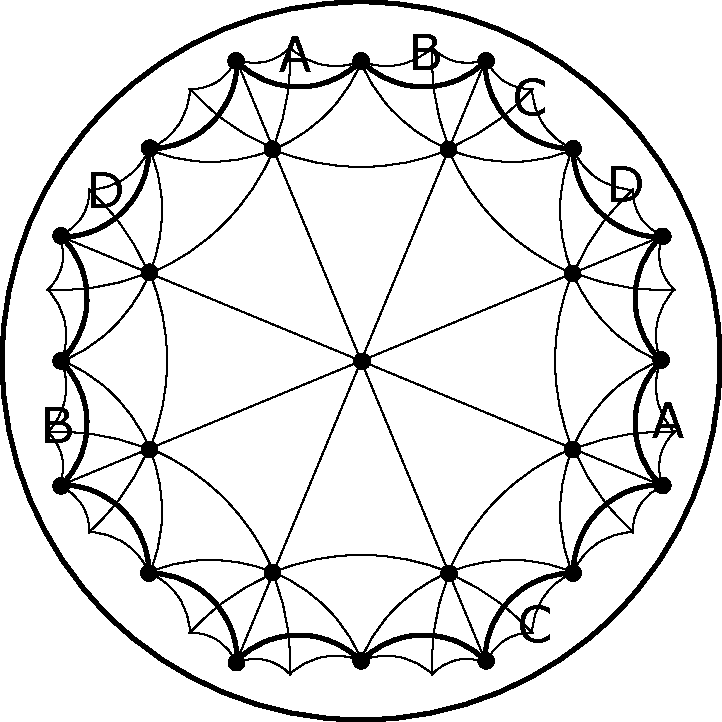
\includegraphics[width=2in]{figures/125_base_.pdf} 
	\caption{Hyperbolic tessellation on $8(1, 2, 5)$}
	\label{fig:125}
\end{figure}

% The euclidean triangles on the fundamental piece of $\Pi$ have a one-to-one correspondence to the hyperbolic triangles.

For each $i,$ there are $\gcd(d, d_i)$ preimages $\widetilde{p_i}$ of $p_i$ on $C.$ Hence, each $\widetilde{p_i}$ is a non-trivial cone point. To pin down a holomorphic 1-form on $C,$ we find cone metrics on $\mathbb{C}\mathbb{P}^1$ and pull-back to its covering. We say that a cone metric on $\mathbb{C}\mathbb{P}^1$ is \textbf{admissible} if its pullback yields a flat structure on $C.$ The following proposition is a version of Gauss-Bonnet theorem.

\begin{proposition} Given a compact Riemann surface of genus $g$ with a cone metric, let $p_1, \ldots, p_n$ be distinguished points with respective cone angles $\theta_i.$ Then $\sum\limits_{i=1}^n \theta_i = 2 \pi (2 g - 2 + n).$
\end{proposition}

Specifically, the sum of cone angles on a genus zero curve is $2 \pi (n - 2).$ Given branching indices such that $\sum\limits_{i=1}^n d_i = d (n - 2),$ we get a cone metric on the Riemann sphere with cone angles $\frac{2 \pi d_i}{d}$ at each $p_i.$ For example, by putting a cone metric on the quotient sphere where the cone angles are $\frac{1 \pi}{4}, \frac{2 \pi}{4},$ and $\frac{5 \pi}{4}$ as in Figure~\ref{fig:125_flat}, one can see that the identification of edges are by translations. In other words, this gives rise to a translation structure on the eightfold cover of the sphere. 

\begin{figure}[htbp] %  figure placement: here, top, bottom, or page
   \centering
   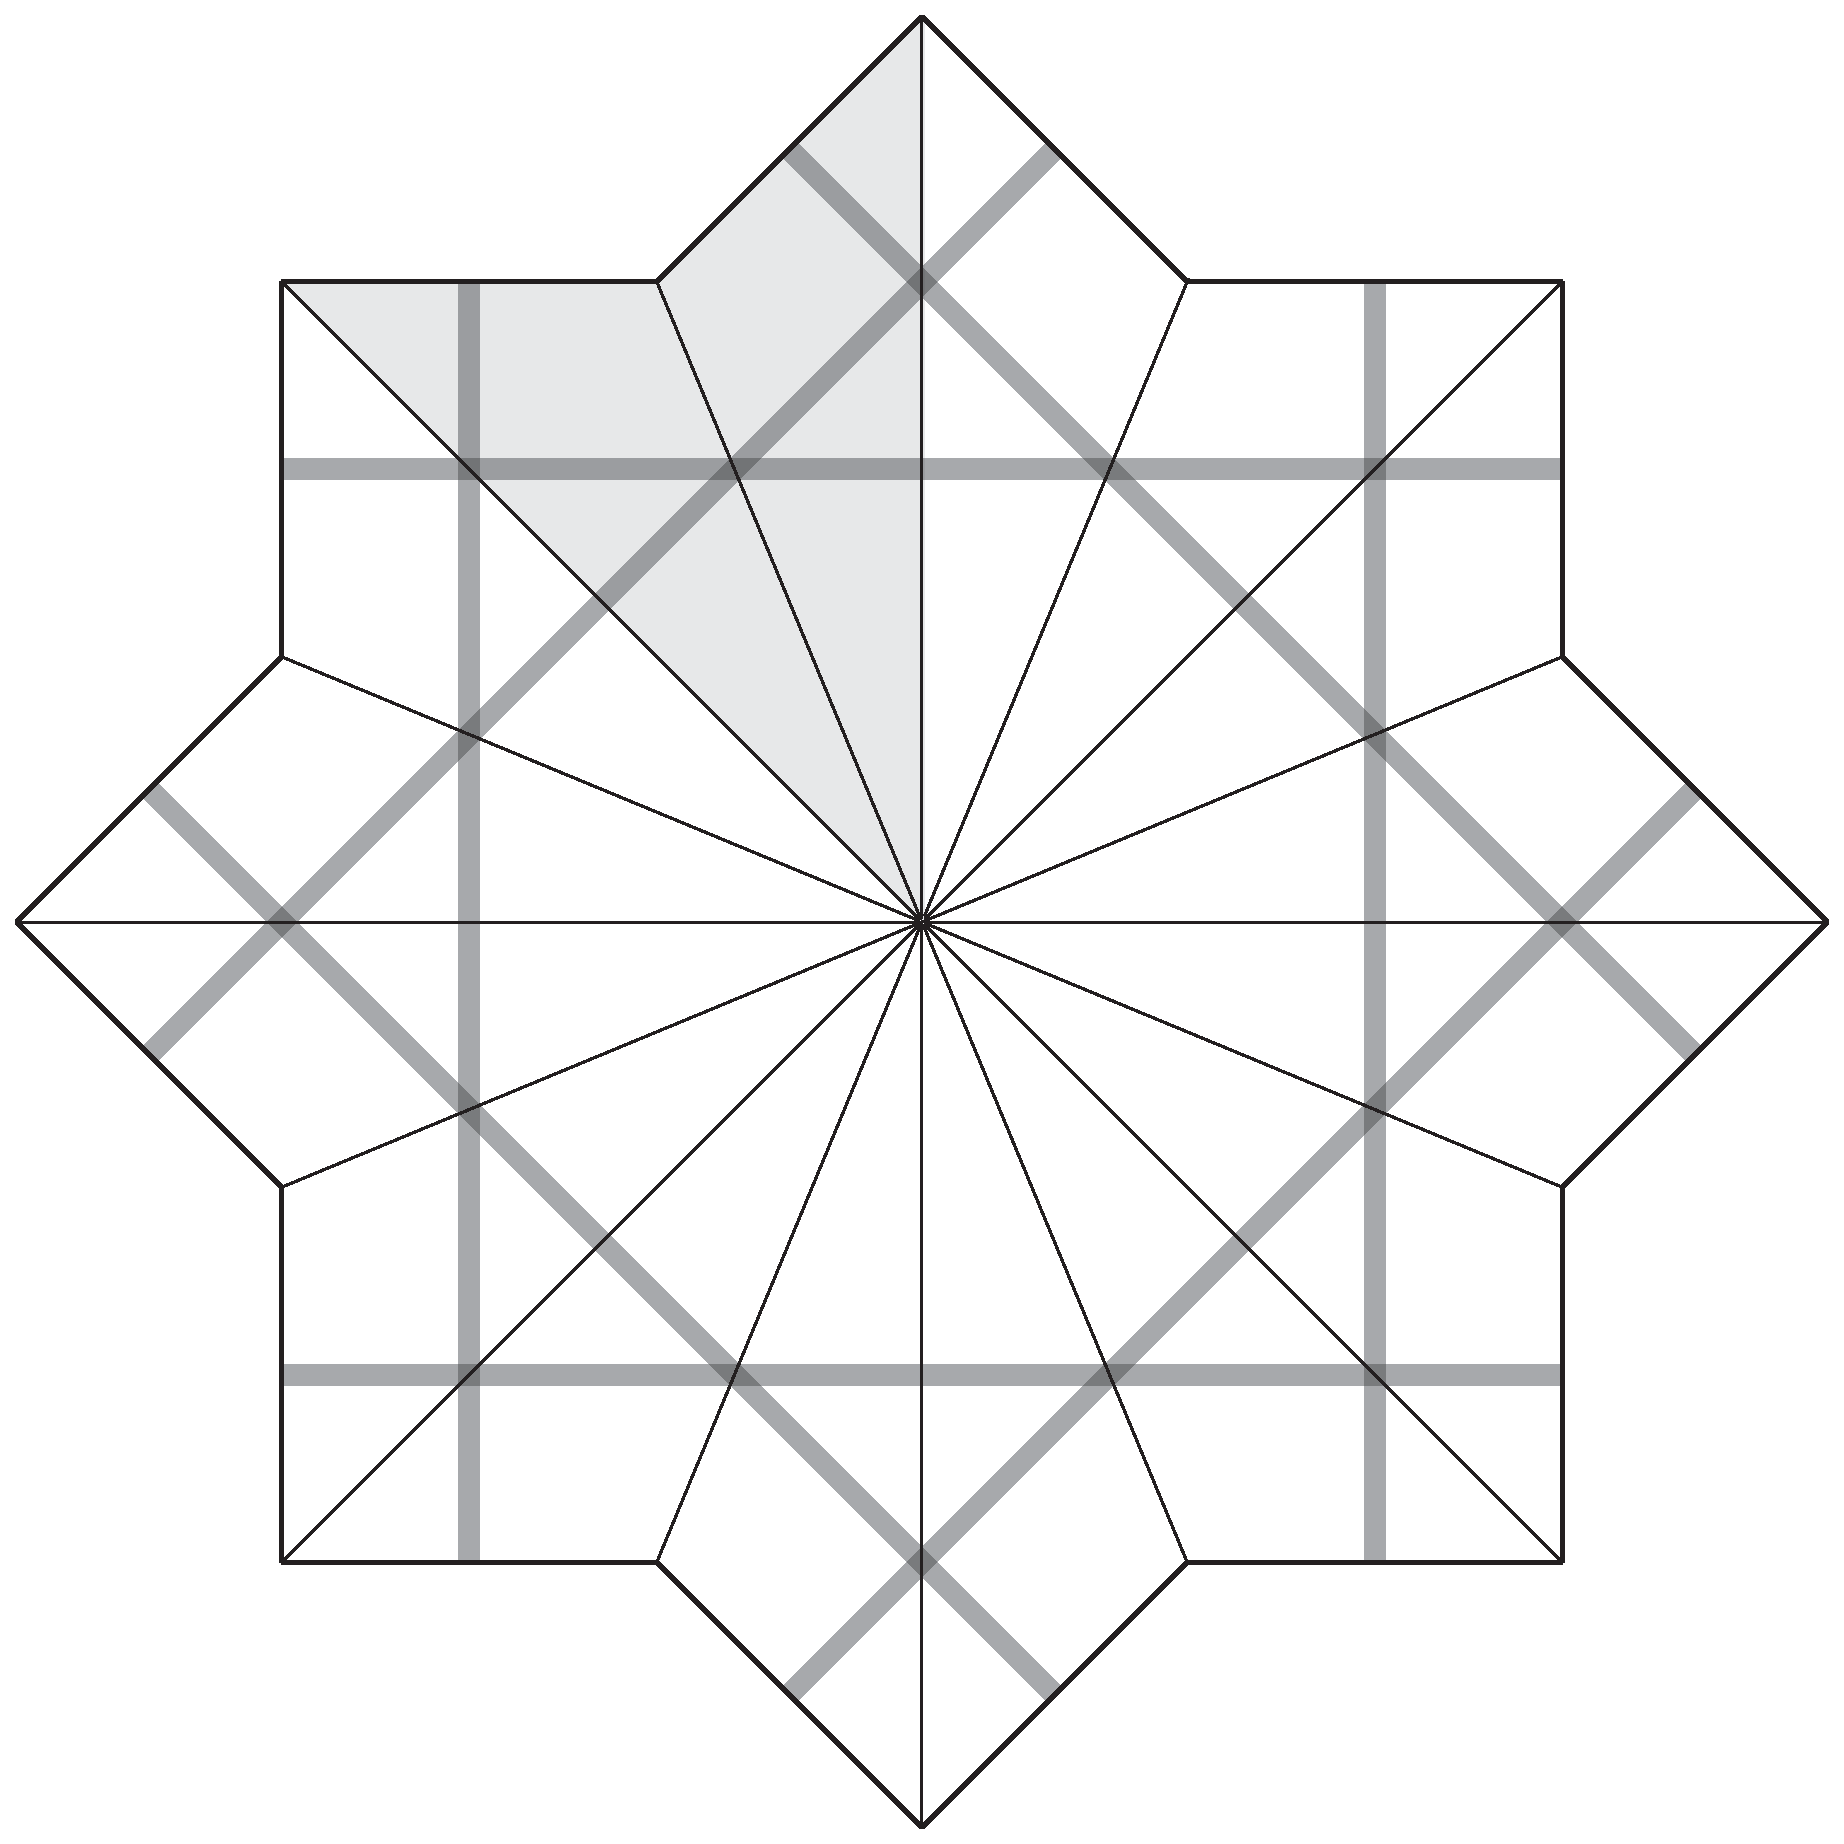
\includegraphics[width=2in]{figures/125_flat.pdf} 
	\caption{A flat structure $\omega_1$ on $8(1, 2, 5)$}
	\label{fig:125_flat}
\end{figure}

In order to compute the Jacobian of the curve, we need a basis of holomorphic 1-forms. Our goal is to find other admissible cone metrics on the sphere that yield different translation structures (linearly independent 1-forms) on the same curve. We claim that the cone metric given by cone angles $\frac{2 \pi a_i}{d}$ where $a_i \equiv d_i \pmod d$ is admissible (Theorem 3.4, \cite{dthesis}). An easier way of finding admissible cone metrics is given by the following notion of multipliers.

\begin{defn} Given branching indices $d (d_1, \ldots , d_n),$ we say $a \in \{1, \ldots, d - 1\}$ is a \textbf{multiplier} if the cone metric given by cone angles $\frac{2 \pi}{d} (a \cdot d_1 \pmod d, \ldots , a \cdot d_n \pmod d)$ is admissible. 
\end{defn}

Theorem 3.5, \cite{dthesis} proves that for $n = 3,$ there are exactly $g$ multipliers. In other words, one achieves a basis of holomorphic 1-forms. 

\subsubsection*{Admissible cone metrics on Octa-4} Given branching indices $8 (1, 2, 5),$ multipliers 1, 2, and 5 give rise to cone metrics with cone angles $\frac{2 \pi}{8}(1, 2, 5),$ $\frac{2 \pi}{8}(2, 4, 2),$ and $\frac{2 \pi}{8}(5, 2, 1),$ respectively. These cone metrics yield a basis of holomorphic 1-forms with the following divisors: $$(\omega_1) = 4 \widetilde{p_3}, \qquad (\omega_2) = \widetilde{p_1} + \widetilde{p_{2_1}} + \widetilde{p_{2_2}} + \widetilde{p_3}, \qquad (\omega_3) = 4 \widetilde{p_1}.$$

For example, Figure~\ref{fig:flat_rs2} presents $\omega_2$ given by cone angles $\frac{2 \pi}{8}(2, 4, 2).$

\begin{figure}[htbp] %  figure placement: here, top, bottom, or page
   \centering
   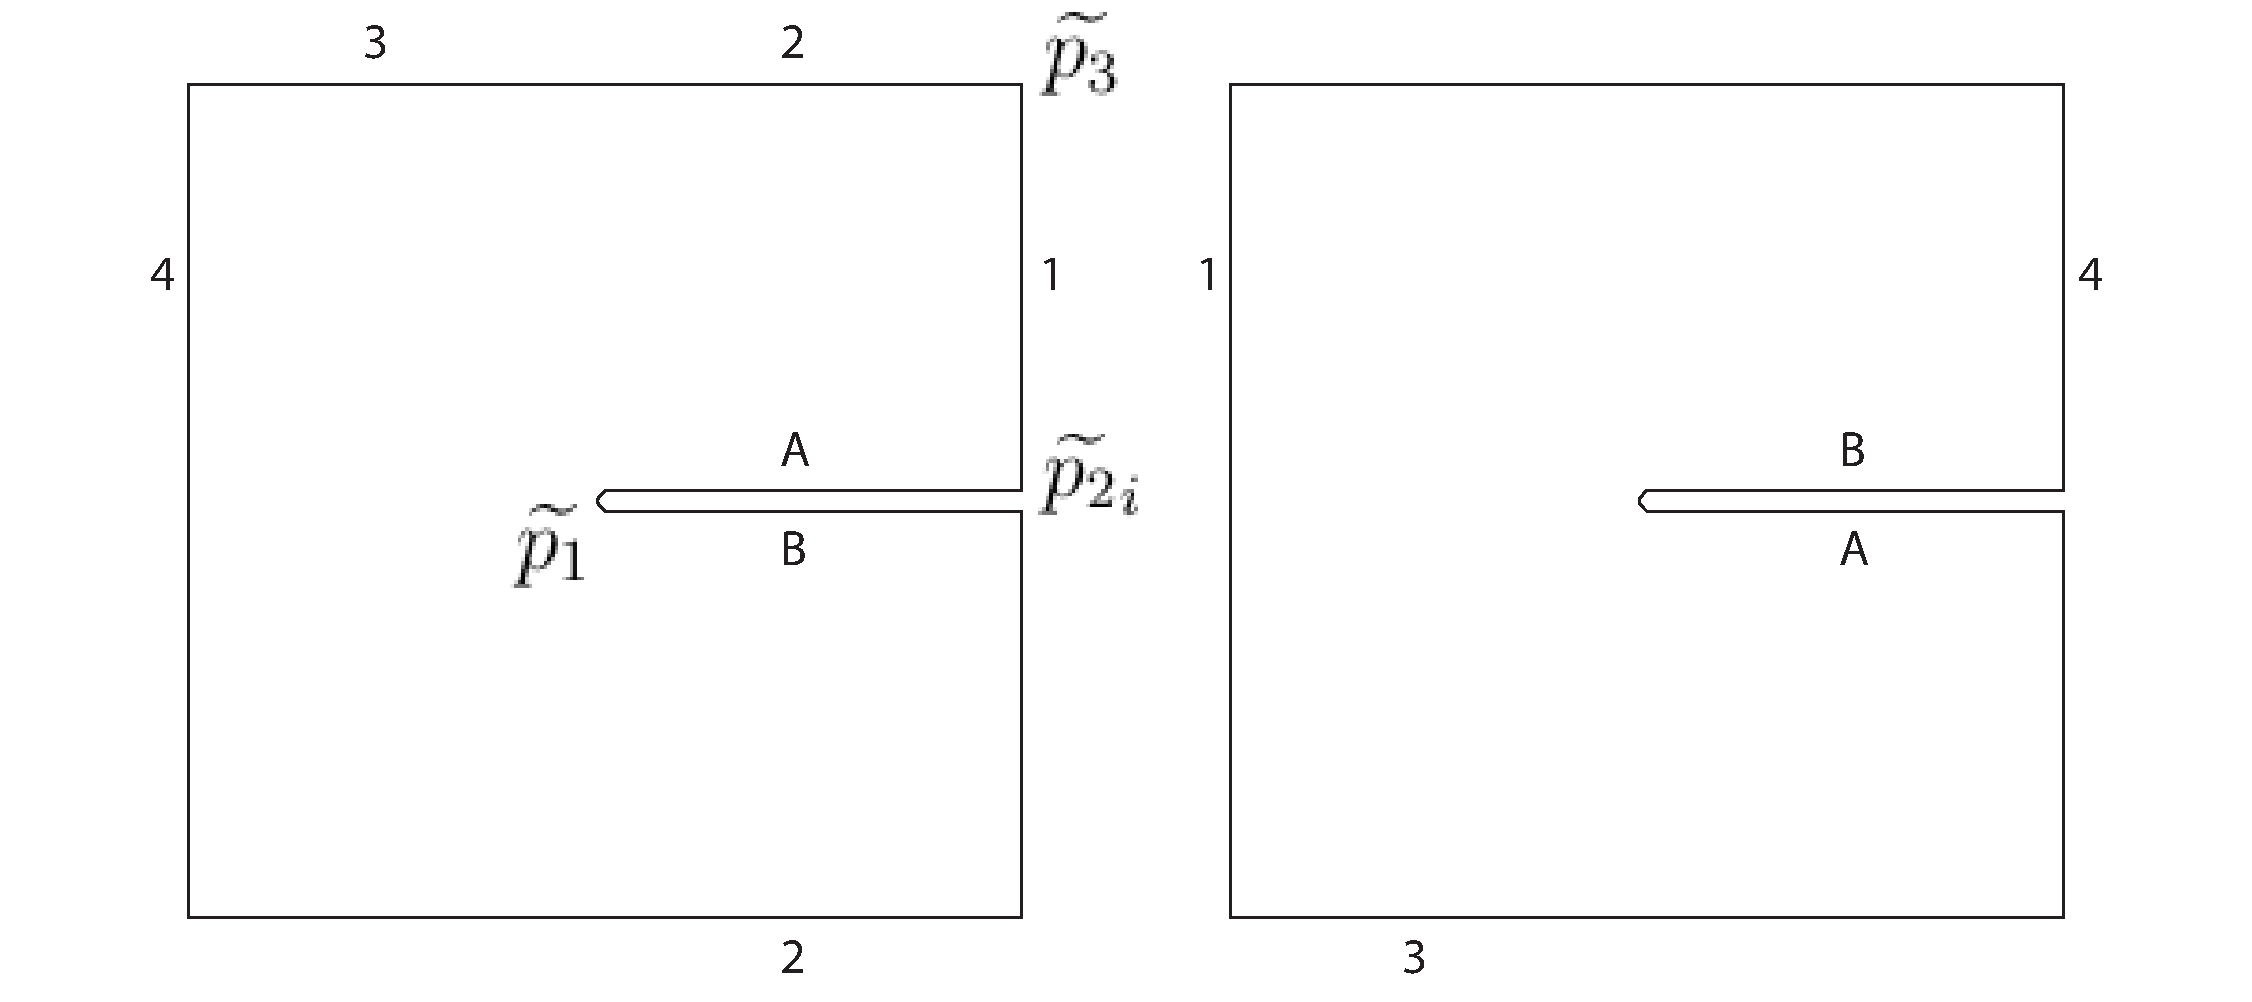
\includegraphics[width=2in]{figures/flat_rs2.pdf} 
	\caption{A flat structure $\omega_2$ on $8(1, 2, 5)$}
	\label{fig:flat_rs2}
\end{figure}


\begin{remark} Note that 3, 6, and 7 are not multipliers as their corresponding forms do not yield canonical divisors. On the other hand, 4 is not a multiplier as the cone metric derived from cone angles $\frac{2 \pi}{8} (4, 0, 4)$ is not admissible. This induces a meromorphic form whose divisor is $3 \widetilde{p_1} - \widetilde{p_2}_1 - \widetilde{p_2}_2 + 3 \widetilde{p_3}.$ \end{remark}



\subsection{Computing the Period Matrix on Cyclic Covers}
\label{sec:cyclicperiod}
In this section, we use the flat structure of a surface to compute the period matrix of a given surface. We will look at the simplest case where $n = 3$ and $d_1 = 1.$ Then, since $\sum d_i = d,$ a cone metric with cone angles $\frac{2 \pi}{d}(d_1, d_2, d_3)$ is admissible. $Y$ is topologically equivalent to a doubled triangle with angles $\frac{2 \pi}{d}(d_1, d_2, d_3)$ so we construct $X$ with $d$ copies of $Y,$ which yields a flat structure on $X.$  We will follow the underlying surface of Octa-4 as our leading example.

\begin{figure}[htbp]
    \centering
    \subfloat[Flat sixteengon represents $\omega_1$]{{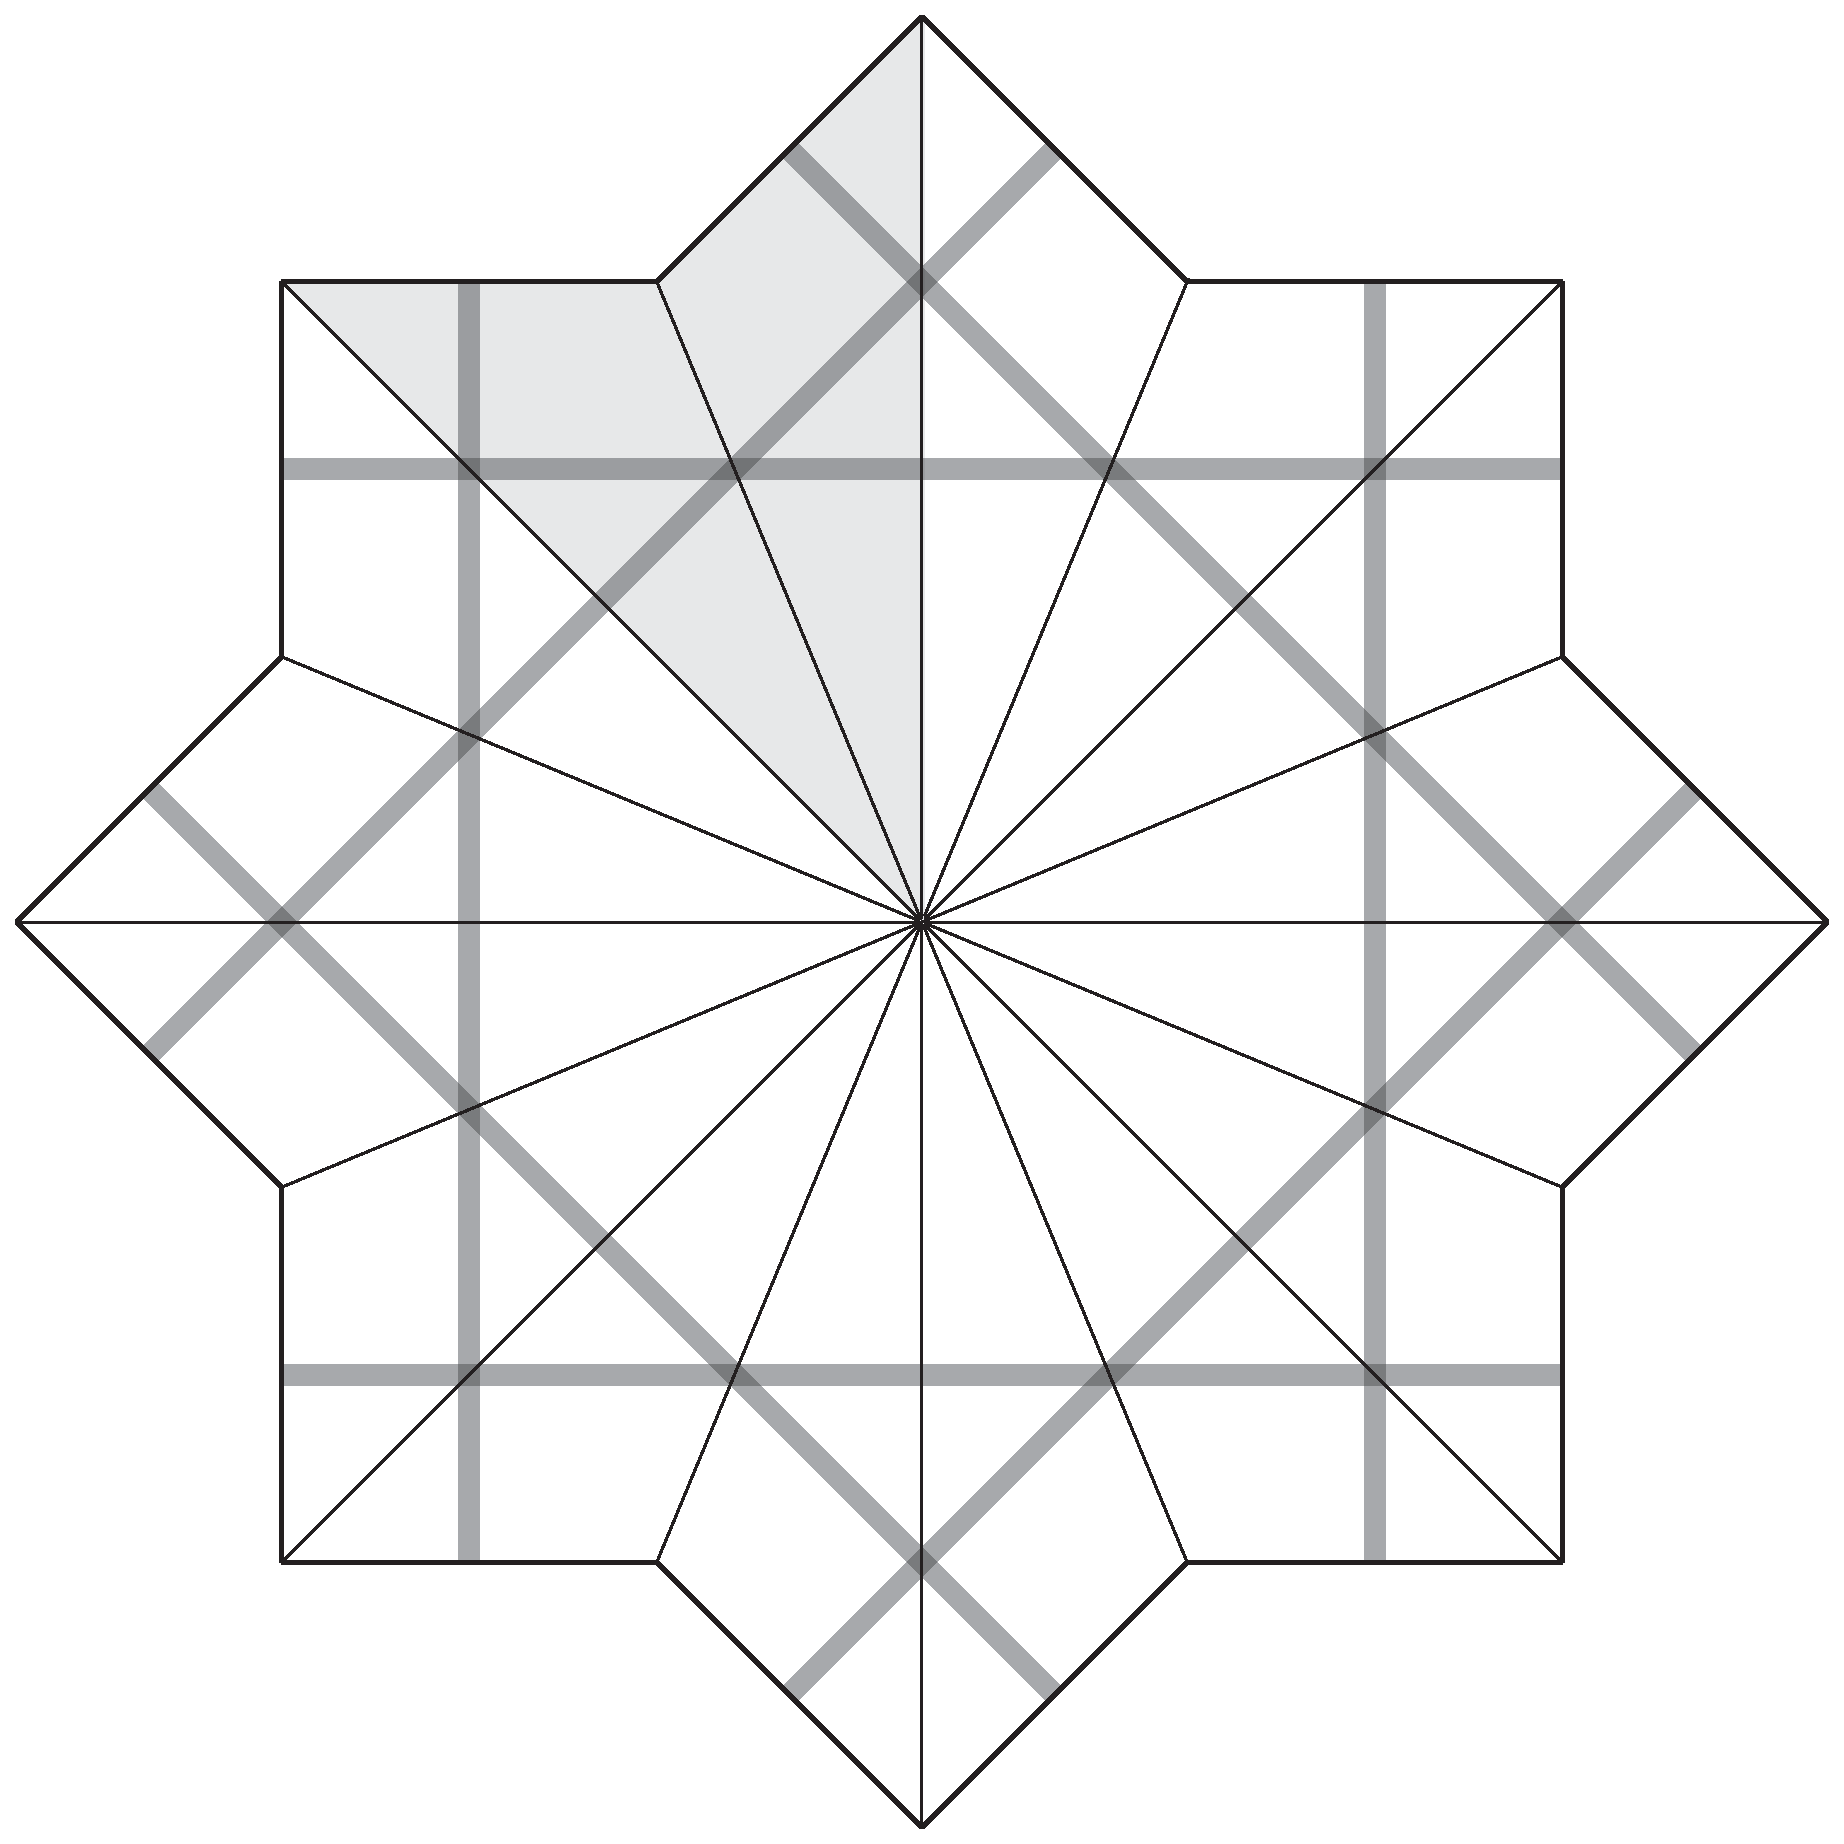
\includegraphics[width=2.75in]{figures/125_flat.pdf}}}
    \qquad
    \subfloat[Representation of $\omega_2$]{{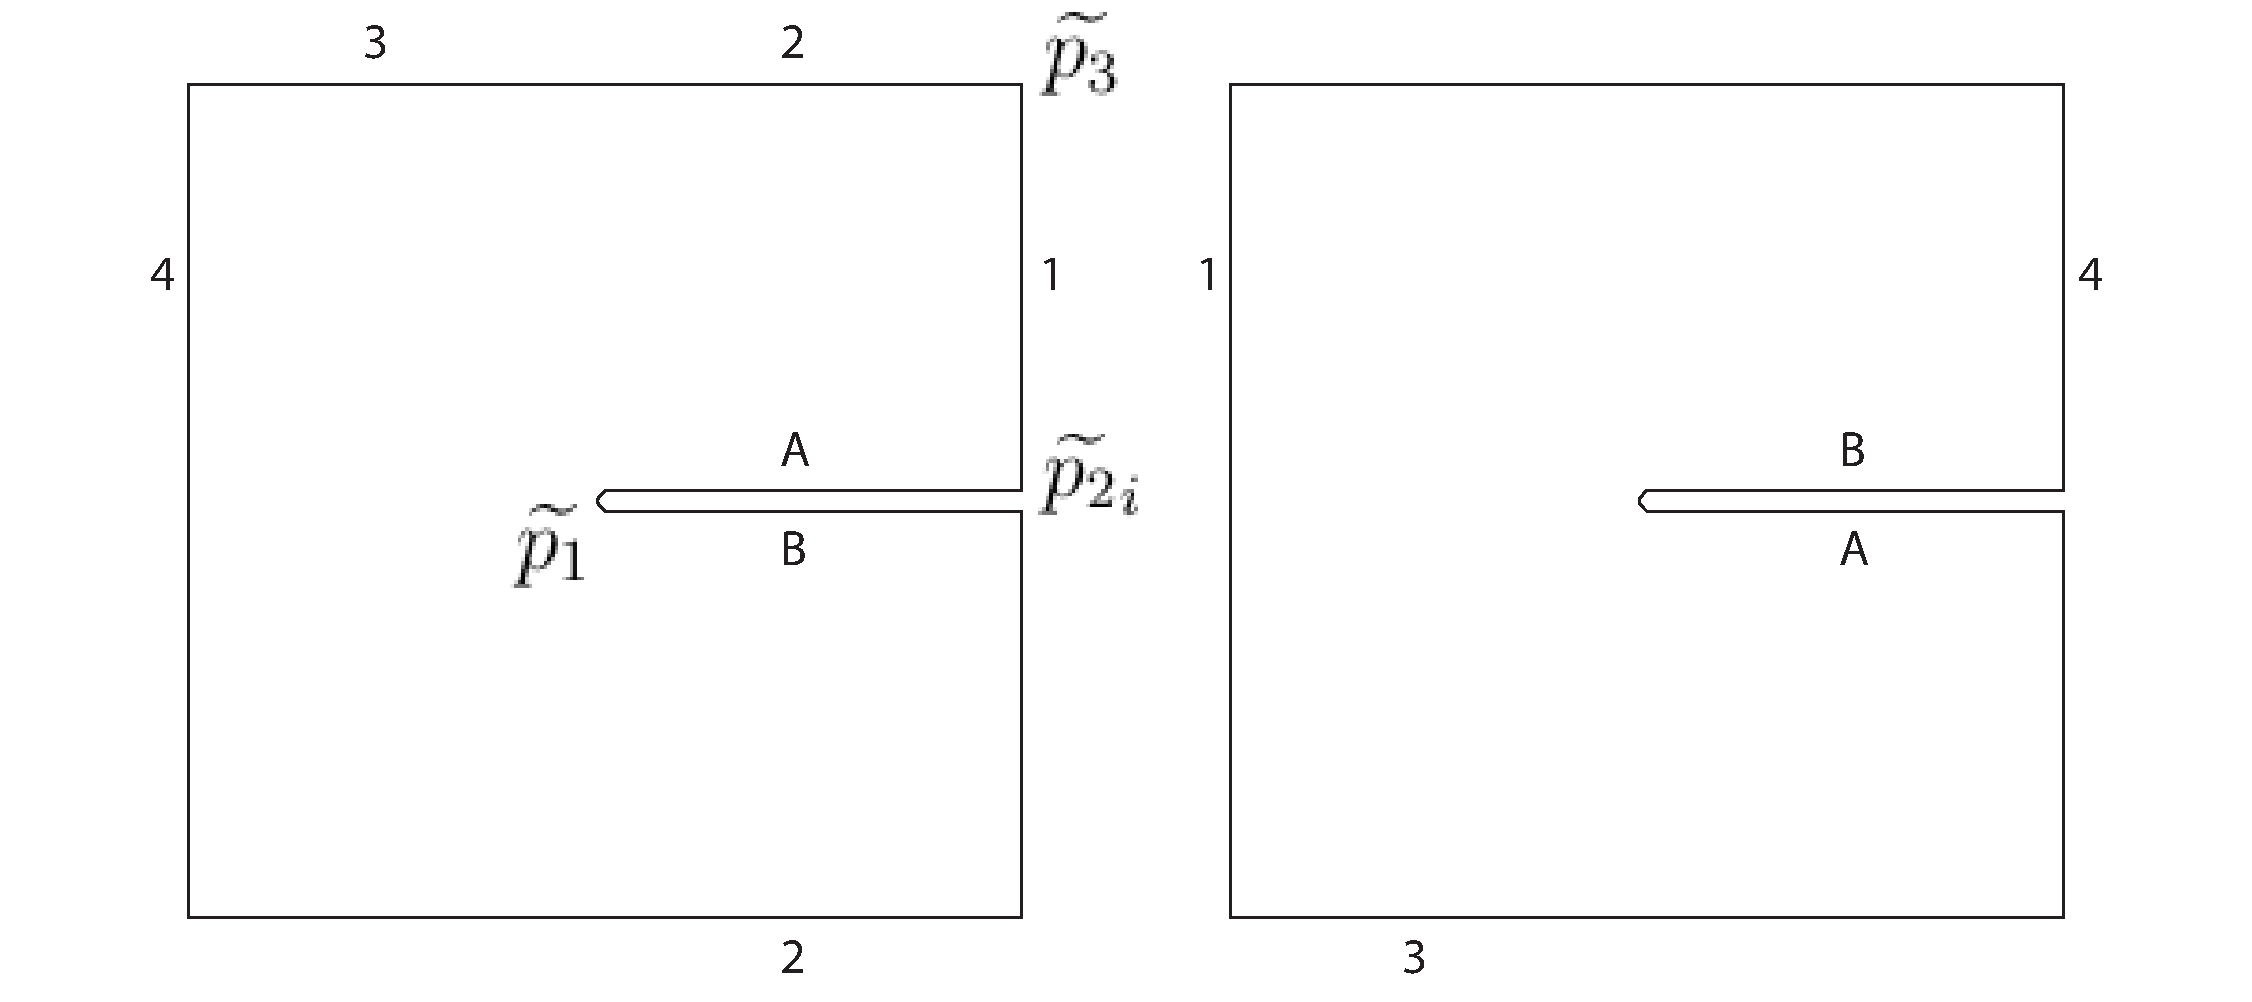
\includegraphics[width=2.75in]{figures/flat_rs2.pdf}}}%
    \caption{8(1, 2, 5)}%
    \label{fig:125}%
\end{figure}

Figure~\ref{fig: 125_flat} shows the flat structures on the underlying surface of Octa-4 \cite{dami}. The identification of edges are via parallel translations, which verifies that the cone metric is admissible. Parallel translations yield closed cycles on the surface from which we get a homology basis with the following intersection matrix

$$\textrm{int}_1 = \begin{pmatrix} 0 & 1 & 1 & 0 & 0 & 0 \\
 -1 & 0 & 1 & 1 & 0 & 0 \\
 -1 & -1 & 0 & 1 & 1 & 0 \\
 0 & -1 & -1 & 0 & 1 & 1 \\
 0 & 0 & -1 & -1 & 0 & 1 \\
 0 & 0 & 0 & -1 & -1 & 0 \end{pmatrix}.$$

Then the period matrix is computed as follows: 
$$\P_1 = \left(
\begin{array}{cccccc}
 1 & e^{\frac{\pi i}{4}} & i & e^{\frac{3 \pi i}{4}} & -1 & e^{-\frac{3 \pi i}{4}} \\
 1 & i & -1 & -i & 1 & i \\
 1 & e^{-\frac{3 \pi i}{4}} & i & e^{-\frac{\pi i}{4}} & -1 & e^{\frac{\pi i}{4}} 
\end{array}
\right)$$

\begin{remark} In \cite{dthesis}, the first author computes the period matrix by choosing a different homology basis. The closed cycles are images of the ``handles'' on the polyhedral surface embedded in $\R^3.$ This yields the following intersection matrix 
$$\textrm{int}_2 = \begin{pmatrix} 0 & 0 & 0 & 1 & 0 & 0 \\
 0 & 0 & 0 & 0 & 1 & 0 \\
 0 & 0 & 0 & 0 & 0 & 1 \\
 -1 & 0 & 0 & 0 & 0 & 0 \\
 0 & -1 & 0 & 0 & 0 & 0 \\
 0 & 0 & -1 & 0 & 0 & 0\end{pmatrix}$$ and the following period matrix

$$\Pi_2 = (A|B) = \begin{pmatrix}  1 - i& -((1 + i)/(1 + \sqrt{2}))& (1 + i)/(1 + \sqrt{2})& 1 + i& \sqrt{2}& 2 - \sqrt{2} \\  -2i& 2i& 2i& 2i& -2& -2\\ -1 - i & (1 - i)(1 + \sqrt{2})& (-1 + i)(1 + \sqrt{2})& 1 - i& i\sqrt{2}& i(-2 - \sqrt{2})  \end{pmatrix} $$ and $$\tau = (A^{-1}B) = \begin{pmatrix}i & \frac{1 + i}{2} & \frac{1 + i}{2}\\
\frac{1 + i}{2} & i & \frac{1 + i}{2}\\
\frac{1 + i}{2} & \frac{1 + i}{2} & i\end{pmatrix}$$
\end{remark}


In general, % emphasize on the fact that this arises from cyclicity
we get 

$$\P_ = \left(
\begin{array}{ccccc}
 1 & e^{\frac{2 \alpha_1 \pi i}{d}} & e^{\frac{4 \alpha_1 \pi i}{d}} & \cdots & e^{\frac{2 (2 g - 1) \alpha_1 \pi i}{d}} \\
 1 & e^{\frac{2 \alpha_2 \pi i}{d}} & e^{\frac{4 \alpha_2 \pi i}{d}} & \cdots & e^{\frac{2 (2 g - 1) \alpha_2 \pi i}{d}} \\
 \vdots
 1 & e^{\frac{2 \alpha_g \pi i}{d}} & e^{\frac{4 \alpha_g \pi i}{d}} & \cdots & e^{\frac{2 (2 g - 1) \alpha_g \pi i}{d}} \\
\end{array}
\right)$$
where $\alpha_i$ are the multipliers.




\subsection{A Non Cyclic Cover: The Modular Curve $X_0(63)$}


\label{sec:modular}
Recall that $SL_2(\Z)$ acts transitively on the upper half plane $\mathfrak{h}$ by $\tau \mapsto \frac{a\tau + b}{c\tau + d}$. We quotient the upper half plane by subgroups $\Gamma$ of $SL_2(\Z)$ and metrize the quotient, however, this yields non-compact Riemann surfaces. To get a compact Riemann surface, we consider the extended upper half plane $\mathfrak{h}^{+} := \mathfrak{h} \cup \R \cup \{ \infty \}$ as a subset of $\C P^1$.  

We are most interested in quotients of the upper half plane $\mathfrak{h}^{+}$ by the following subgroups of $SL_2(\Z)$. These subgroups come up naturally in the study of modular forms associated to elliptic curves.

\begin{defn} 
\begin{align*} 
\Gamma_0(N) &:= \left\{ \begin{pmatrix} a & b \\ c & d \end{pmatrix} \in SL_2(\Z) \text{ }  \Big| \text{ } \begin{pmatrix} a & b \\ c & d \end{pmatrix} \equiv  \begin{pmatrix} * & * \\ 0 & * \end{pmatrix} \mod N \right\} \\
\Gamma_1(N) &:= \left\{ \begin{pmatrix} a & b \\ c & d \end{pmatrix} \in SL_2(\Z) \text{ }  \Big| \text{ }  \begin{pmatrix} a & b \\ c & d \end{pmatrix} \equiv  \begin{pmatrix} 1 & * \\ 0 & 1 \end{pmatrix} \mod N \right\} \\
\Gamma(N) &:= \left\{ \begin{pmatrix} a & b \\ c & d \end{pmatrix} \in SL_2(\Z) \text{ }  \Big| \text{ }  \begin{pmatrix} a & b \\ c & d \end{pmatrix} \equiv  \begin{pmatrix} 1 & 0 \\ 0 & 1 \end{pmatrix} \mod N \right\}
\end{align*}
 \end{defn} 

% The automorphism groups of $X(N)$ were found in \cite{bwx} to be $PSL_2(\Z/N\Z)$ (when the genus is greater than 2). The case of all $X_1(N)$ was reportedly found in general in a print, but the second author cannot locate the answer nor a copy of this manuscript. 
The automorphism groups of $X_0(N) := \mathfrak{h}^{+} / \Gamma_0(N)$ were calculated in \cite{km} except for $N=63$. The case of $X_0(63)$ was resolved 2 years later by Elkies in \cite{elkies} by two different proofs: a conceptual one that uses enumerative geometry and the modular structure, and an explicit one that exhibits the modular equations. Our method would work for any $N$, we exposit the case of $N=63$ due to its late blooming history.

%\begin{conjecture} \label{63conj}  All principal polarizations on a Jacobian $J$ coming from curves are found by the method discussed in section ~\ref{sec:find}.  In other words: if there are exactly $n$ curves such that $J \simeq \Jac(C_1) \simeq \Jac(C_n)$, where $C_i \nsimeq C_j$ when $i \neq j$, then the algorithm will find at least the canonical principal polarizations on $J$ associated to $C_1, ..., C_n$.\end{conjecture} 

\begin{conjecture} \label{63conj} The program \texttt{CullPB.m} finds all principal polarizations on the curves we consider. \end{conjecture}

If this conjecture is true, it would be a radically different proof than that of Elkies, since we approach by computing the automorphism group of the Jacobian of $X_0(63)$. Assuming this conjecture, we have

\begin{thm*} $\Aut(X_0(63)) \simeq S_4 \times \Z/2$ \end{thm*} 

\begin{proof} Note the following theorem from \cite{km}: 

\begin{lemma*} $\Aut(X_0(63))$ is either $A_4 \times \Z/2$ or $S_4 \times \Z/2$. 
\end{lemma*}

Using the period matrix provided by Mascot, performed with 150 precisions, \texttt{autperio.sage} (using Conjecture ~\ref{63conj}) gives

\begin{lemma*} $\Aut(X_0(63))$ is either $C_2^{\text{ }4}$ or $S_4 \times \Z/2$.
\end{lemma*}

Therefore, it must be that $\Aut(X_0(63)) \simeq S_4 \times \Z/2$. 
\end{proof} 
%add citation for this paper etc. 

\vspace{+10pt} 
The period matrix used in our calculation of $\Aut(\Jac(X_0(63)), p_i)$ was computed by Nicolas Mascot using an alteration of his personal code.

\begin{remark} Mascot, in \cite{n}, discusses finding the period matrices for $X_1(N)$ by integrating cuspforms along modular symbols. His algorithm works for any compactified modular curve, but it works best when $N$ is square-free. In the non-squarefree case, the coefficients in the $q$-expansions of the cuspforms and the $j$-invariant do not converge as quickly, thus they require more digits of precision. \end{remark}

\begin{remark} In private correspondence, John Voight programmatically proved that $X_0(63)$ is not a cyclically branched cover of the sphere. Given that the genus of the quotient $X_0(63)/H$ is equal to the dimension of the $H$-invariant differentials, he shows that the list of dimensions of the space of $H$-invariant differentials on $X_0(63)$ (where $H$ is a cyclic subgroup of $Aut(X_0(63))$) does not contain zero. 
 \end{remark} 





 \section{Programmatically Computing the Automorphism Group of Plane Curves and Abelian Varieties over $\mathbb{C}$}



\begin{remark} The first two subsections of the section are copied from section 4 of Bruin-Sijsling-Zotine \cite{jeroen} with lots of exposition and examples added for the readers' convenience. This sets us up to introduce the code for brute force calculating principal polarizations. All of our code is available at \begin{center}\texttt{https://github.com/catherineray/aut-jac}\end{center} We discuss the certification of these numerical results in Section ~\ref{cert}. \end{remark} 

Let us examine abelian varieties represented as analytic groups $X := V/\Lambda$ and $X' := V'/\Lambda'$. They need not be Jacobians.

%\begin{remark} We slightly abuse notation here, $\Lambda$ represents both a matrix in $M_{g \times 2g}(\Z)$, and the $2g$-integral-dimensional (i.e., $g$-complex-dimensional) lattice in $\C^g$ generated by the columns of that matrix.\end{remark}
 
%A homomorphism $\phi: J \to J'$ induces a tangent map $V \to V'$ and a map on ``homology"\footnote{In the case of Jacobians $\Jac(C) = H^0(C, \Omega_{C}^1)/H_1(C; \Z) \simeq \C^g/\Lambda$, hence the name homology representation for the map on $\Lambda$.} $\Lambda_1 \to \Lambda_2$. After a choice of basis, these correspond to matrices $T=T_\phi \in M_{g_2 \times g_1}(\C)$ and $R = R_\phi \in M_{2g_2 \times 2g_1}(\Z)$. 

%Let $\Lambda_1 = (A \mid B)$, that is, break the gx2g matrix into two square matrices.



\begin{thm*}[BL 1.2.1] Let $X:= V/\Lambda$ and $X':= V'/\Lambda'$ be abelian varieties. Under addition the set of homomorphisms $\Hom(X, X')$ forms an abelian group. There is an injective homomorphism of abelian groups: 


\begin{align*} 
\rho: \Hom(X, X') &\to \Hom(V, V') \\
f &\mapsto F
\end{align*} 

The restriction to the lattice $\Lambda$ is $\Z$-linear, thus we get an injective homomorphism: 


\begin{align*} 
\rho|_{\Lambda}: \Hom(X, X') &\to \Hom_{\Z}(\Lambda, \Lambda') \\
f &\mapsto F|_{\Lambda}
\end{align*} 


\end{thm*}
%Let $E := \begin{pmatrix} 0 & I \\ -I & 0 \end{pmatrix}$, in other words, the standard symplectic matrix.

We will namely use the representation $\rho|_{\Lambda}$ and find the basis of our set of maps in terms of this representation. 

We work in the category of varieties equipped with principal polarizations, which we discuss in section~\ref{sec:intropol}. In this category, morphisms are morphisms of pairs. That is,

$$f: (X, c_1(\mc{L})) \to (Y, c_1(\mc{M}))$$

such that $f^*(Y, c_1(\mc{M})) = (X, c_1(\mc{L}))$ (for isomorphisms).  We may represent polarizations as integral valued alternating forms. 

% tktk 
% define polarization here before using it in the next definition


\begin{defn} Let $a$ be a polarization of $X$. We call $\Aut(X, a)$ a \textbf{symplectic automorphism group} of $X$, as it respects the symplectic form $a$. 
\end{defn}

% tktk 
% Define/mention what R is here. You use it in the algorithm but there's no info about that here. 

Let $E_1$ and $E_2$ be forms representing $c_1(\mc{L}_1)$ and $c_1(\mc{L}_2)$, respectively. Note that a map $\alpha: (X_1, c_1(\mc{L}_1)) \to (X_2, c_1(\mc{L}_2))$ such that $$\alpha^*(c_1(\mc{L}_2)) = c_1(\mc{L}_1)$$ is equivalent to $R$ in the image of $\rho|_{\Lambda}$ such that $$R^tE_2R = E_1$$


\subsection{Computing the Automorphism Group of Plane Curves}
\label{sec:autplane}

\begin{remark} This section is on the algorithm used in \texttt{autplane.sage}. \end{remark}

In the case that our abelian variety is of the form $\Jac(C_i) =: J_i$, and we know the curve $C_i$, there is a special principal polarization $E_i$ with respect to that curve $C_i$. This is programmatically found using Lemma 2.6 from \cite{jeroen}. 
\vspace{+10pt} 
%The following psuedocode is copied from section 4.2 ``Computing symplectic isomorphisms" \cite{jeroen}  for the readers convienience. Note that steps 4-7 coicide with steps (???) in the previous algorithm, however, since the canonical principal polarizations are known, we use only one iteration of steps 5-7. We write it out to avoid unneccessary confusion.


%or equivalently, $\alpha_*(c_1(\mc{L})) = c_1(\mc{M})$.

\textbf{Algorithm:} Compute the set of isomorphisms between curves. 

\textit{Input:} Planar equations $f_1$, $f_2$ for curves $C_1$, $C_2$.\n
$\text{}$ $\hspace{2mm}$\textit{Output:} The set of isomorphisms $C_1 \to C_2$, or the group $\Aut(C)$ if $C_1 = C_2$.

\begin{enumerate}
\item Check if $g(C_1) = g(C_2)$; if not, return the empty set.
\item Check if $C_1$ and $C_2$ are hyperelliptic; if so, use the methods in \cite{hyp}.
\item Determine the period matrices $P_1, P_2$ of $C_1, C_2$ to the given precision.
\item Determine a $\Z$-basis of $\Hom(J_1, J_2) \subset M_{2g \times 2g}(\Z)$ represented by integral matrices $R \in  M_{2g \times 2g}(\Z)$. [Lemma 4.3 \cite{jeroen}]
\item Using Fincke-Pohst\footnote{This is an algorithm for finding vectors of small norm. We use it here to solve for the finite set of solutions $R = \sum_{i = 1}^{2g} \lambda_i B_i$, where $B$ is the basis from step 4.}, determine the finite set [from 5.1.9 BL] $$S = \{ R \in \Hom(J_1, J_2) \text{ } | \text{ } \text{tr}((E_1^{-1}R^tE_2)R) = 2g\}$$
\item Return the subset\footnote{The condition $R^tE_2R = E_1$ (i.e., $E_1^{-1}R^tE_2R = \text{Id}$) implies that $\text{tr}((E_1^{-1}R^tE_2)R) = 2g$. So we first solve for the latter to thin the results, then solve for the former from that set.}  of $R \in S$ which further satisfies $R^tE_2R = E_1$. (These are the symplectic endomorphisms.)
\item Look at the subset of $R$ such that $\det(R) = \pm 1$. These are the symplectic automorphisms.
\item If $J_1 = J_2$, find the group structure of this subset.
%Using the canonical morphisms with respect to the chosen basis of differentials, return the subset of elements of $S$ that indeed induce an isomorphism $J_1 \to J_2$.
\end{enumerate}

\vspace{+10pt} 

Note that if the curves $C_1$ and $C_2$ are non-hyperelliptic, by the precise Torelli theorem, we get $\Hom((J_1, E_1), (J_2, E_2)) \simeq \Hom(C_1, C_2) \sqcup \{ \pm 1 \}$ from this algorithm. So, we must remove the direct summand $\{ \pm 1 \}$.

\begin{remark} Step 8 of the above algorithm was added by the second author to tame these unwieldy matrix groups, and is achieved as follows.\end{remark}

\textbf{Algorithm:} Compute the group structure of an underlying set of matrices.

\textit{Input:} A set of matrices which are a group by multiplication. \n $\text{}$ $\hspace{2mm}$\textit{Output:} The group structure of the set.

\begin{enumerate}
\item Check cardinality of the set. Call this $N$.
\item Take first 15 elements of the set, use GAP to check if these generate a matrix group $G$ of the correct order $N$. If not, it generates a group of order $K$, where $KM = N$. Take more elements of order dividing $M$ until they generate a group of the correct order.
\item Use \texttt{IdGroup(G)} in GAP.
\end{enumerate}

\subsection{Computing the Automorphism Group of Abelian Varieties}
\label{sec:autperio}

\begin{remark} This section is on the algorithm used in \texttt{autperio.sage} \end{remark}

\begin{notation} Let $A:= V/\Lambda$ be an abelian variety of dimension $g$. Let $e_1, ..., e_g$ be the chosen basis for $V$, and $\lambda_1, ..., \lambda_{2g}$ be a corresponding chosen basis for $\Lambda$. Let $\Pi$ be the corresponding period matrix such that $A := \C^g/\Pi \Z^{2g}$.
\end{notation}

\textbf{Algorithm:} Compute the group of isomorphisms between abelian varieties. 

%what makes these automorphisms symplectic? 

\textit{Input:} Period matrices of abelian varieties $J_1$ and $J_2$, as $\Pi_1$ and $\Pi_2$ respectively. \n
$\text{}$ $\hspace{2mm}$\textit{Output:} For each combination of principal polarizations $(a_i, b_j)$, the set of isomorphisms between $(J_1, a_i)$ and $(J_2, b_j)$ (or the group, if they coincide).
\begin{enumerate}
\item Check if $g_1 = g_2$; if not, return the empty set.
\item Determine a $\Z$-basis of $\Hom(J_1, J_2) \subset M_{2g \times 2g}(\Z)$ represented by integral matrices $R \in  M_{2g \times 2g}(\Z)$.
\item Find many principal polarizations $\{a_i\}$ and $\{b_j\}$ for $J_1$ and $J_2$ respectively using \texttt{CullPB} (exposited in the next section).
\item Apply steps 5-8 of the previous section substituting each pair $(a_i, b_j)$ for $(E_1, E_2)$. For each pair, this will produce the set of isomorphisms between $(J_1, a_i)$ and $(J_2, b_j)$.
\item If $(J_1, a_i) = (J_2, b_i)$, find the group structure of each set $\Aut(J_1, a_i)$ (using the algorithm in the previous section).
\end{enumerate}


%what makes these automorphisms symplectic? 

%\begin{remark} This algorithm is a repeat of the algorithm in the next section, beginning with different inputs [it begins at step (4) of the algorithm for plane curves]. We exposit it seperately to emphasize that is works for more than just plane curves. \end{remark}


%In the following description of the program, we assume that the period matrix is already known. We find the period matrix using either Lee-Webers's method for cyclic covers \todo{does it work more generally?}, or using Bruin's calculation of the period matrix from the Voronoi cell decomposition.


\subsection{Certifying Heuristic Methods}
\label{sec:cert}
We summarize here the fantastic work of Costa-Mascot-Sijsling-Voight \cite{rigor} on certifying that numerically computed endomorphisms of a Jacobian are infact endomorphisms of that Jacobian. This is extremely nontrivial because in an analytic sense, abelian varieties with no principal polarizations are dense in the moduli space (of Big Period Matrices) (SOURCE?). 

A key conceptual part of their approach is relating divisors on $X \times Y$ to endomorphisms of the Jacobians $\Jac(X)$ and $\Jac(Y)$ via the theory of correspondences. All endomorphisms of Jacobians come from correspondences. Each correspondece on $X \times Y$ induces a homomorphism of the divisor groups of $X$ and $Y$. These homomorphisms in turn induce homomorphisms of Jacobians. In our case, $X=Y$, but we will exposit the more general case. Let $C$ be a prime divisor on $X \times Y$, then we denote the associated correspondence as follows.

\begin{center}
\begin{tikzcd}
  & X \times Y \arrow[ld, "\pi_1^C"'] \arrow[rd, "\pi_2^C"] &   \\
X &                                                         & Y
\end{tikzcd}
\end{center}

\begin{center}
\begin{tikzcd}
                                                       & \Div(C) \arrow[rd, "(\pi_2^C)_*"] &         \\
\Div(X) \arrow[ru, "(\pi_1^{C})^*"] \arrow[rr, dashed] &                                   & \Div(Y)
\end{tikzcd}
\end{center}

\begin{center}
\begin{tikzcd}
                                                       & \Jac(C) \arrow[rd, "(\pi_2^C)_*"] &         \\
\Jac(X) \arrow[ru, "(\pi_1^{C})^*"] \arrow[rr, dashed] &                                   & \Jac(Y)
\end{tikzcd}
\end{center}


reference the rest to their endo paper.



Given a pair of .,..?
show that there is a divisor which vanishes on a set of points associated to the numerical endomorphism. 


Their method is along the lines of the following: \begin{itemize} 
\item we get a matrix M which is a tangent representation, associated to this M we have some points $\tilde{Q_j}$ by either Newton/Puiseux lifting. 
\item We can then check if there is a divisor E which fits those points, and then further make a "better" divisor Y that also fits these points? (where Y is just E with no exciting nilpotents in the intersection of irreducible dim 1 components) 
\item If yes, since divisor = morphism of Jacobians, we get an honest endomorphism. 
\end{itemize}

\subsubsection{From Simple to Non-simple}

While we are on the topic of correspondences, we wish to make a remark on how to use techniques for simple varieties to bound below the number of principal polarizations of nonsimple varieties. Our program does not use this, but it is useful for context.

\begin{remark} Since every abelian variety is isogenous to a product of simple abelian varieties $$A \simeq A_1 \times ... \times A_k$$ it is reasonable to ask how the numbers of principal polarizations on $A_i$ are related to that of $A$. 

Let's quickly establish some vocabulary to discuss this intuitively. Recall that we may also define a principal polarization on $A$ as an isogeny which is also an isomorphism between $A \to A^\vee$, where $A^\vee$ denotes the dual variety. Let $A$ and $B$ be arbitrary abelian varieties. Note that $\text{Corr}(A, B) \simeq \Hom(B, A^\vee)$, where we take a correspondence from $A$ to $B$ to be a line bundle $\mathcal{L}$ over the product $A \times B$ which is trivial when restricted to $A$ or $B$.

We are interested in $\Aut(A, A^\vee)$, which is isomorphic to $\Corr(A, A)^\times$ but the problem of comparision arises immediately and obviously without having to pass to isomorphisms. %We wish to compare $$\Hom\left(\prod_{i= 1}^k A_i, (\prod_{j= 1}^k A_j)^{\vee}\right) \qquad \text{ and  } \qquad \prod_{i, j} \Hom(A_i, A_j^{\vee})$$

We wish to compare

$$\Corr\left(\prod_{j= 1}^k A_j, \prod_{i= 1}^k A_i\right) \qquad \text{ and  } \qquad \prod_{i, j} \Corr(A_j, A_i)$$

Let $C$ and $D$ be abelian varieties. Given a line bundle on $C$ and on $D$, we get a line bundle on $C \times D$, but not vice-versa. Intuitively, the product $C \times D$ may have many more interesting cycles than the product of the cycles of $C$ and $D$, and may not necessarily restrict to a line bundle on $C$ or $D$. Therefore, in general the number of principal polarizations of $A$ is at least the product of the principal polarizations of the simple components $A_i$, that is, $$\pi(A_1 \times ... \times A_k) \geq \prod_{i=1}^k \pi(A_i)$$ as observed. %We saw that $\Jac(\text{I-WP})$ is isogenous to a product of 4 elliptic curves. Since these curves are all isomorphic, we only get one principal polarization from this decomposition, but we found at least 9 principal polarizations on their product.
\end{remark}  



\subsection{Introduction to Polarizations: From Theory to Code}
\label{sec:intropol}
The notion of a polarization of an abelian variety has many faces. If a complex torus has a polarization, it is an abelian variety.

\begin{defn} A \textbf{polarization} of a complex torus $X$ is an embedding $j: X \to \P^N$ for large enough $N$. \end{defn}


%is it important that it is a projective embedding

We can understand this embedding $j$ as a map $$p \mapsto [a_1(p) : \cdots : a_{N-1}(p)]$$ where $a_i$ are a chosen generating set of global sections of a line bundle $\mc{L}$ on $X$. 

%locally free of rank 1 globally generated sheaf = ample line bundle; are other ranked globally generated sheaves going to give other embeddings? 

\begin{defn} A line bundle $\mc{L}$ is defined to be \textbf{very ample} on $X$ if it defines a closed embedding into $\P^N$ for large enough $N$. %if it has finitely many global sections, such that for every $x \in X$, there is at least one section not vanishing at this point. 
\end{defn}

\begin{defn} A line bundle is \textbf{ample} if a tensor power of the line bundle is very ample. Since the Chern class is additive, $c_1(\mc{L}^{\otimes k}) = kc_1(\mc{L})$, the ample bundle and its tensor power are equivalent datum. \end{defn} 

\begin{remark} In other words, $\mc{L}$ is defined to be ample if it (or a tensor power of it) specifies an embedding of $X$ into projective space.\end{remark}

%Note that $\mc{F}$ is a sheaf generated by its finitely many global sections. We may restate this property as follows. 

%\begin{remark} Let $X$ be a Riemann surface of genus $g$. We can understand this embedding $j$ as the map $$p \to [\omega_1(p) : \cdots \omega_g(p)]$$ where $\omega_i$ are a chosen basis of holomophic differentials on $X$, that is, a chosen generating set of global sections of a line bundle (the sheaf of differential 1-forms). This is where we get the canonical polarization associated to a curve. \end{remark}
%This embedding information is often specified by \todo[inline]{IS IT EQUIVALENT TO} an ample line bundle $\mc{L}$ on $X$. 

\begin{defn} Line bundles $\mc{L}_1$ and $\mc{L}_2$  on $X$ are \textbf{analytically equivalent} if there is a connected complex analytic space $T$, a line bundle $\mc{L}$ on $X \times T$, and points $t_1, t_2 \in T$ such that $$\mc{L} |_{X\times \{t_i\}} \simeq \mc{L}_i$$ for $i = 1, 2$. \end{defn}

A line bundle $\mc{L}$ over $X$ is specified up to analytic equivalence by its first Chern class $c_1(\mc{L}) \in H^2(X; \Z)$. More precisely,

\begin{thm*} 
[2.5.3 BL] Let $X$ be an abelian variety. For line bundles $\mc{L}_1$ and $\mc{L}_2$ over $X$, the following statements are equivalent: 
\begin{enumerate} 
\item $\mc{L}_1$ and $\mc{L}_2$ are analytically equivalent.
%\item $\mc{L}_1 \otimes \mc{L}_2^{-1} \in \text{Pic}^0(X)$
\item $c_1(\mc{L}_1) = c_1(\mc{L}_2)$
%\item $\phi_{\mc{L}_1} = \phi_{\mc{L}_2}$
\end{enumerate}
\end{thm*}


%We may recover a line bundle $\mc{L}$ on $X$ from its first chern class by $(f, c_1(\mc{L}))^*(\mc{P}_X) \simeq \mc{L}^{\otimes 2}$, where $\mc{P}_X$ is the Poincare correspondence on $X$.  


%and a semi-character $\chi$.  \ti{add more on semicharacter, is it needed to fully specify polarization}


\begin{defn} The \textbf{first Chern class} of a line bundle $\mc{L}$ is the image of $\mc{L} \in \Pic(X) = H^1(\mc{O}_X^*)$ under the map $c_1$ on cohomology which arises as follows. Consider the exact sequence $$0 \to \Z \to \mc{O}_X \to \mc{O}_X^* \to 0$$ and its long cohomology sequence:
%\to H^1(X, \Z) \to H^1(\mc{O}_X) \to 
$$\cdots \to H^1(\mc{O}_X^*) \xrightarrow{c_1} H^2(X, \Z) \to \cdots$$ \end{defn} 

%\ti{is there a more universal defn?} 


%pp works for all varieties, why are algebraic varieties abelian?

%\ti{why is chern class of line bundle automatically integral by [BL B.1 and 2.1.1]?}, because that is its target!!!

%By definition, every (chern class of a holomorphic) line bundle on $X$ \in H^2(X, \Z)

We associate to every first Chern class an alternating form.

\begin{thm*} [BL 1.3.2 \& 2.1.2] $$\psi: H^2(X; \Z) \simeq \Alt^2(\Lambda, \Z)$$ 
\end{thm*} 



%To each element of $S$, 

%This associates to every (chern class of a holomorphic) line bundle on $X$  
%\ti{explore this because the code in 4.4 doesn't seem to reflect this, what small combinations is CullPB using to check if it has det 1?? how is CullPB checking thm 10?} 
 
 
Let $S$ be the set of $c_1(\mc{L})$ where $\mc{L}$ ranges over all holomorphic line bundles on $X$. The image $\psi(S)$ is isomorphic to all Hermitian alternating forms.

%\begin{remark} We may use the Frobenius form to calculate all Hermitian forms and prune out those which are in $\phi(S)$. \end{remark}


%It is specifically the Hermitian forms which come from line bundles represented as maps $X \to \hat{X}$ (this representation is explained in section???).

\begin{thm*} [BL 2.1.6] Let $X:= V/\Lambda$ be an abelian variety. For an alternating form $E: V \times V \to \R$, the following conditions are equivalent: 

\begin{enumerate} 
\item There is a holomorphic line bundle $\mc{L}$ on $X$ such that $\psi(c_1(\mc{L}))= E$. 
\item $E(\Lambda, \Lambda) \subseteq \Z$, and $$E(iv, iw) = E(v, w)$$
\end{enumerate}
\end{thm*} 

 
\begin{remark} Note that from each element $\Alt^2(\Lambda, \Z)$ we obtain via $\R$-linear extension an alternating form $\Alt^2(V, \R)$ (as in rational versus analytic representation, see [BL 1.2.1]). We also have an isomorphism between real valued forms satisfying 2.1.6(2) and Hermitian forms. \end{remark}

It is important to emphasize that not all forms satisfying 2.1.6(2) correspond to Chern classes of ample line bundles. Ampleness is stronger than holomorphicity, hence we need a stronger condition. 

\begin{defn} 
A line bundle $\mc{L}$ on $X$ is called \textbf{positive} if $c_1(\mc{L})$ is represented by a positive-definite Hermitian form.
\end{defn}

\begin{thm*} 
Let $X$ be a smooth complex projective variety. A line bundle $\mc{L}$ on $X$ is ample if and only if it is positive.
\end{thm*}

%We end our descent from theory to practice with the test for how to check if an alternating integral form is Hermitian.

%\begin{remark} By [BL 2.1.7], the alternating forms over $\R$ of 2.1.6 are the imaginary parts of hermitian forms over $\C$. That is, there is a bijection between the set of Hermitian forms on $V$ and the set of real valued alternating forms on $V$ satisfying $E(iv, iw) = E(v, w)$. \end{remark} 

This is how we ask the computer to find polarizations of an abelian variety $X$, which are steps 1 and 2 of the following section.

However, there may be infinitely many polarizations. We are interested in a particular kind of polarization.

\begin{defn}  A polarization $c_1(\mc{L})$ of $X$ is called \textbf{principal} if $\mc{L}$ has only one section up to constants, i.e. $\dim H^0(X, \mc{L}) = 1$.  \end{defn} 

As a motivational theorem:

\begin{thm*} [BL 4.1.2] Every polarization is induced by a principal polarization via an isogeny. \end{thm*}

By Narasimhan-Nori \cite{nn}, there are only finitely many principal polarizations on a variety $X,$ which is irreducible and smooth. And as a corollary, only finitely many curves may have the same Jacobian since each non-isomorphic curve gives a non-isomorphic principal polarization on its Jacobian.


\begin{comment}
\begin{defn} 
The \textbf{Jacobian} of a genus $g$ curve $C$ is defined as quotient space $V/\Lambda$. Here $V$ is the dual of the $g$-complex dimensional vector space of global holomorphic differentials on $C$, i.e. $H^0(C, \Omega_{C/\C}^1) \simeq H^1(C, \mc{O}_C)$, and $\Lambda$ is the lattice of all elements of $V$ of the form $[\gamma]: \omega \mapsto \int_{\gamma} \omega$, where $\gamma$ is a closed curve in $C$. In other words, $\Jac{C} := H^0(C, \Omega_{C, \C}^1)^*/H_1(C)$.
\end{defn} 

\begin{remark} The Jacobian is an ``abelianization" functor from $\Jac: \text{RiemSurf} \to \text{AbVar}_{\C}$. \end{remark}

A curve gives a principal polarization on its Jacobian as follows. We are given an intersection form which takes $\cap: H_1(X, \Z) \times H_1(X, \Z) \to \Z$ (computing the intersection number of two given cycles). 

\begin{remark} We may pick a \end{remark}

We may construct a form $H: H^{1, 0}(C, \C) \times H^{1, 0}(C, \C) \to \Z$ by precomposing $\cap$ with a dualizing map. That is, $H$ takes a pair of forms, returns the dual of each form as a cycle, and computes the intersection of these cycles using $\cap$. By the earlier discussed [BL 2.1.6], this Hermitian form gives a polarization. 

\begin{remark} It is difficult to recover the line bundle corresponding $\mc{L}$ to this polarization $c_1(\mc{L})$ as the inverse to the first Chern class map is very difficult to construct.\end{remark}

\end{comment}

\subsection{Finding Principal Polarizations} 
\label{sec:find}
We begin with a representation of our abelian variety as $A := \C^g/\Pi\Z^{2g}$. 

Then $\Lambda$ is the associated lattice spanned by the columns of $\Pi$. Thus, we have a distinguished basis for the homology of $A$, corresponding to the columns of $\Pi$. 

%\todo[inline]{Do I want to elaborate on this? This is a program, and in a program, we must pick a basis.}

\vspace{+5pt}

\textbf{Algorithm:} Compute many principal polarizations on a given abelian variety $A$.

\textit{Input:} An abelian variety $A := \C^g/\Pi\Z^{2g}$, where $\Lambda$ is the associated lattice to the period matrix $\Pi$. \n
$\text{}$ $\hspace{2mm}$\textit{Output:} Many principal polarizations on $A$.
\begin{enumerate} 

\item The magma function \texttt{FindPolarizationBasis} determines all integral alternating pairings $E$ on the homology, i.e., $E\in \Alt^2(\C^g, \Z)$, for whose real extension we have:

$$E (i v, i w) = E (v, w)$$
This is a basis of alternating forms $\{E_i\}$.
\item Check that $E$ is positive-definite.
\item \texttt{CullPB.m} tries some small combinations and sees if $E_i$ actually gives a pairing with determinant 1 indicating that $E_i$ is a principal polarization. If so, it returns $E_i$. This gives us a set $\{E_k\}$ of integral pairings on the homology.
\item For each $i$, we rewrite these pairings in a symplectic basis. That is, we find a basis of $\Lambda$ in which $$E_i = \begin{pmatrix} 0 & D \\ -D & 0 \end{pmatrix}$$ where $D = \text{diag}(d_1, ..., d_g)$ which we may do by the elementary divisor theorem (section 3.1, \cite{bl}). 

\end{enumerate} 

\begin{remark} This does nothing but modify the (homology) basis of $\Lambda$. Multiplying $\Pi$ on the right with this integral matrix, we get a new period matrix $Q$ whose columns span exactly the same lattice but for which the standard symplectic pairing $E$ is actually the Chern class of a line bundle. This is often called the Frobenius form of the period matrix $\Pi$. \end{remark}


%\footnote{Note that every period matrix $\Pi$ may be written as $(\tau \mid Id)$ where $\tau$ is symmetric with positive definite imaginary part.} We then normalize the left part of $Q$ to be 1. This gives us $\tau$. What do we use tau for then?



%\item As a last step, we check that things (?? do we in fact do this earlier?) are positive definite, to make sure that the aforementioned line bundle is ample.



\section{Studying Principal Polarizations via Automorphisms of the Jacobian}

%how is frobenius form like elementary divisors for alternating integer matrices.?

\begin{defn} We say two principal polarizations $p_1$ and $p_2$ on $A$ are \textbf{auto-equivalent} if and only if $\Aut(A, p_1) \simeq \Aut(A, p_2)$. \end{defn}

Our program produces many auto-equivalent principal polarizations.  Note that auto-equivalence is a weaker notion of equivalence than analytic equivalence, as discussed in section ~\ref{sec:questions}. 

If the abelian variety is indeed a Jacobian, this method will in practice return at least enough polarizations to find the canonical principal polarization. As we discussed in the introduction, it is an unsolved problem to find all possible principal polarizations associated to a given abelian variety, called ``explicit Narasimhan-Nori". 

%(maybe talk about relation to automorphism group?)


%\ti{discuss the interest in this problem, previous work, provided examples, waiting on MO post!!! and mention the I-WP example as being unsolved}

%https://math.stackexchange.com/questions/2837906/is-there-one-canonical-principal-polarization-of-a-jacobian-per-nonisomorphic-cu, and Observations Regarding Different Curves with the Same Jacobian https://mathoverflow.net/questions/303803/an-example-of-curves-with-the-same-jacobian-but-different-jacobian-automorphism


\subsection{Examples}
\label{sec:accident}

\begin{cat} Insert some text here introducing examples. \end{cat}

\begin{table}[!hbt]
\caption{Automorphism Groups wrt each of the Principal Polarizations}
\centering
\begin{tabular}{ l | c c r r r} \hline
  \shortstack{Curve C} & Genus & \shortstack{\# Principal \\ Polarizations} & $\Aut(\Jac(C), a_i)$ & $|\Aut(\Jac, a_i)|$ & GAPID \\ \hline\hline
  Klein & 3 & 2 & $S_4 \times C_2$ & 48 & [48, 48]\\ 
  & & & $GL_3(F_2) \times C_2$ & 336 & [336, 209] \\  \hline %N
Fermat & 3 & 2 &  $(C_4\wr C_2) \times C_2$ & 64 & [64, 101] \\ %N 
& & & $(C_4^{\text{ }2} \rtimes S_3) \times C_2$ & 192 & [192, 944] \\  \hline
$12(1, 5, 6)$ & 3 & 3 & $D_6$  & 12 & [12, 4]\\ %12, ?
&  & & $C_4 \times S_3$ & 24 & [24, 5] \\
& & & $C_4 \times D_4$ & 32  & [32, 25] \\ \hline 
Bring & 4 & 2 & $C_2^{\text{ }2} \times D_4$ & 32 & [32, 46] \\
& & & $C_2 \times S_5$ & 240 & [240, 189] \\ \hline %N 
I-WP & 4 & 9 & $C_2^{\text{ }4}$ & 16 & [16, 14] \\
 
& & & $C_2^{\text{ } 2} \times C_6$  & 24  & [24, 15] \\
 
& & & $C_2^{\text{ } 2} \times D_4$  & 32 & [32, 46] \\
 
& &   & $C_2^{\text{ }3} \times C_6$ & 48 &  [48, 52] \\
 
%& & & $D_4^{\text{ }2}$ & 64 & [64, 226] \\

& & & $C_2^{\text{ }2}\times S_4$ & 96 & [96, 226] \\

& & & $C_6 \times S_4$ & 144 & [144, 188] \\

& & & $(C_2 \times C_6) \times (C_3 \rtimes D_4)$  & 288 & [288, 1002]  \\

& & & $C_3 \times (((C_6 \times C_2) : C_2) \times D_8)$ & 576 & [576, 7780] \\ 

& & & $C_6 \times (S_3 \times ((C_6 \times C_2) : C_2))$ & 864 & [864, 4523] \\ \hline

$X_0(63)$ & 5 & 2 & $C_2^{\text{ }5}$ & 32 & [32,51] \\
& & & $C_2 ^{\text{ }2} \times S_4$ &  96 & [96, 226] \\ \hline
\end{tabular}
\label{table:tablelabel}
\end{table}

\begin{remark} Note that the University of Bristol's GroupNames database at the time of writing has groups up to order 500 with full names and structure description. In the cases where the order is greater than 500, we use the output of \texttt{StructureDescription(G);} \end{remark}

The file containing the period matrices for the above objects is located on \texttt{github/...}.

\subsection{Questions and Answers on Abelian Varieties with Multiple Principal Polarizations}
\label{sec:questions}

We speak here of polarizations up to auto-equivalence and ask natural questions on Jacobians with multiple principal polarizations, answering all but one of the questions using methods developed in our paper.

We fix some notation. Let $\theta_C$ be the canonical principal polarization of $\Jac(C)$ with respect to $C$. We call $\Aut(A, a_i)$ a symplectic automorphism group of $A$, as the automorphisms respect the principal polarization $a_i$, which is a symplectic form on $A$.

\begin{question} $\Aut(\Jac(C), \theta_C)$ will have the highest order of all symplectic automorphism groups of $\Jac(C)$. \end{question}

This is proven false by example $12(1,5,6)$, where $|\Aut(\Jac(12(1, 5, 6)), \phi_{12(1, 5, 6)})| = 24$, but $|\Aut(\Jac(12(1, 5, 6)), a_i)| = 32$ is achieved. It is more dramatically proven false by Schoen's I-WP Surface, where $|\Aut(\Jac(\text{I-WP}), \phi_{\text{I-WP}})| = 288$, but $|\Aut(\Jac(\text{I-WP}), a_i)|$ achieves $576$ and $864$.

\begin{question} Principal polarizations $p_1$ and $p_2$ are auto-equivalent if and only if they are analytically equivalent. In other words, $$\Aut(X, p_1) \simeq \Aut(X, p_2) \Leftrightarrow p_1 = p_2$$ \end{question}

The direction ($\Leftarrow$) is clear because $\mc{L}$ and $\mc{M}$ are analytically equivalent if and only if $c_1(\mc{L}) = c_1(\mc{M})$ by [BL 2.5.3]. The other direction ($\Rightarrow$) is false.  This is proven false by applying our method to the the following two \textit{non-isomorphic} curves with the same (unpolarized) Jacobian from Theorem 1 of \cite{howe1}:

$$X: 3y^2 = (2x^2- 2)(16x^4 + 28x^2 + 1)$$ 

$$X': -y^2 = (2x^2 + 2)(16x^4 + 12x^2 + 1)$$ 

which both have $\Aut(\Jac(X), \theta_X)\simeq C_2 \times C_2 \simeq \Aut(\Jac(X'), \theta_{X'})$. %This is true for many curves in Howe's first family where $t \in \Z^\times$. 

%First, note that $$\Aut(\Jac(X), c_1(\mc{L})) \simeq \Aut(\Jac(X), c_1(\mc{M}))$$ does not immediately imply that $c_1(\mc{L}) = c_1(\mc{M})$.

\begin{question} If $\Jac(C) \simeq \Jac(C')$ as complex varieties, then $$\Aut(\Jac(C), \theta_C) \simeq \Aut(\Jac(C'), \theta_{C'})$$  \end{question} 

We checked this question on the family of hyperelliptic cases of genus 2 from \cite{howe1} Theorem 1, where it is true. However, there is no reason to expect this to be true in general. Yet, we cannot disprove it easily. 


% tktk 
% change this to conjecture if we are not providing an answer

\begin{thebibliography}{20}

\bibitem{bl} 
C. Birkenhake, H. Lange, 
\textit{Complex Abelian Varieties},
Springer, 2004.

\bibitem{rigor}
E. Costa, N. Mascot, J. Sijsling, J. Voight
\textit{Rigorous Computation of the Endomorphism Ring of a Jacobian}
\texttt{https://arxiv.org/pdf/1705.09248.pdf}

\bibitem{jeroen}
N. Bruin, J. Sijsling, A. Zotine,
\textit{Numerical Computation of Endomorphism Rings of Jacobians},
\texttt{https://arxiv.org/pdf/1807.02605.pdf}, preprint.

\bibitem{smith}
B. Smith
\textit{Explicit Endomorphisms and Correspondence, PhD Thesis 2005}

\bibitem{elkies}
N. Elkies,
\textit{The automorphism group of the modular curve $X_0(63)$},
Composito Mathematica,
Vol. 74, 1986, pp.127--152.

\bibitem{fk}
H. Farkas, I. Kra,
\textit{Riemann Surfaces},
Springer-Verlag, New York, 1992.

\bibitem{howe1}
E. Howe,
\textit{Constructing Distinct Curves with Isomorphic Jacobians},
Journal of Number Theory,
Vol. 56, Issue 2, 1996, pp.381--390.

\bibitem{howe2} 
E. Howe,
\textit{Infinite families of pairs of curves over $\Q$ with Isomorphic Jacobians},
Journal of the London Mathematical Society,
Vol. 72, Issue 2, 2005, pp.327--350.

\bibitem{iko}
T. Ibukiyama, T. Katsura, F. Oort,
\textit{Supersingular curves of genus two and class numbers},
Composito Mathematica,
Vol. 57, No. 2, 1986, pp.127--152.

\bibitem{kw}
H. Karcher, M. Weber,
\textit{On Klein's Riemann Surface},
The Eightfold Way, MSRI Publications, 
Vol. 35, 1998, pp.9--49.

\bibitem{km}
M. A. Kenku, F. Momose,
\textit{Automorphism Groups of the modular curves $X_0(N)$},
Composito Mathematica,
Vol. 65, No. 1, 1988, pp.51--80.

\bibitem{sl}
Z. Laing, D. Singerman,
\textit{Transitivity on Weierstrass Points}
Annales Academiae Scientiarum Fennicae Mathematica,
Vol. 37, 2012, pp.285--300

\bibitem{several} 
H. Lange,
\textit{Abelian Varieties with Several Principal Polarizations},
Duke Mathematical Journal,
Vol. 55, Number 3, 1987, pp.617--628.

\bibitem{newlange}
H. Lange
\textit{Principal Polarizations on Products of Elliptic Curves}
\texttt{https://arxiv.org/pdf/math/0508458.pdf}

\bibitem{dami} 
D. Lee,
\textit{On a triply periodic polyhedral surface whose vertices are Weierstrass points},
Arnold Mathematical Journal, 
Vol. 3, Issue 3, 2017, pp.319--331.

\bibitem{dthesis} 
D. Lee, 
\textit{Geometric realizations of cyclically branched coverings over punctured spheres},
\texttt{https://arxiv.org/abs/1809.06321}, preprint.

\bibitem{hyp}
R. Lercier, C. Ritzenthaler, J. Sijsling,
\textit{Fast computation of isomorphisms of hyperelliptic curves and explicit Galois descent},
Proceedings of the Tenth Algorithmic Number Theory Symposium, 2013, pp. 463–-486.

\bibitem{n}
N. Mascot,
\textit{Computing modular Galois representations},
Rendiconti del Circolo Matematico di Palermo,
Vol. 62, Issue. 3, 2013, pp.451--476.

\bibitem{nn} 
M. S. Narasimhan, M. V. Nori,
\textit{Polarisations on an abelian variety},
Proceedings of the Indian Academy of Sciences,
Vol. 90, 1951, pp.125--128.


\bibitem{matti} 
M. Weber,
\textit{Kepler's small stellated dodecahedron as a Riemann surface},
Pacific Journal of Mathematics, 
Vol. 220, 2005, pp.167--182.


\end{thebibliography}
\end{document}

